\documentclass[12pt,a4paper]{article}

% Page setup
\usepackage[a4paper,top=1in,bottom=1in,left=0.5in,right=0.5in]{geometry}
\usepackage{setspace}
\onehalfspacing

\usepackage{etoolbox}
\usepackage[nonumberlist]{glossaries}
\usepackage{hyperref}
\usepackage{graphicx}
\usepackage{float}
\usepackage{xcolor}
\usepackage{colortbl}

% Table packages
\usepackage{array}
\usepackage{booktabs}
\usepackage{longtable}
\usepackage{tabularx}
\usepackage{multirow}
\usepackage{multicol}

% List formatting
\usepackage{enumitem}

% Dotted lines package
\usepackage{dashrule}

% Thai language support
\usepackage{xunicode}
\usepackage{xltxtra}

% Optimized fonts for Thai language - using Medium weight
\setmainfont[
    Path=./font/Sarabun/,
    UprightFont=*-Regular,
    BoldFont=*-Medium,
    ItalicFont=*-Italic,
    BoldItalicFont=*-MediumItalic,
    Scale=1.0,
    Ligatures=TeX,
    WordSpace=1.2,
    PunctuationSpace=1.1
]{Sarabun}

\newfontfamily\thaifont[
    Path=./font/Sarabun/,
    UprightFont=*-Regular,
    BoldFont=*-Medium,
    ItalicFont=*-Italic,
    BoldItalicFont=*-MediumItalic,
    Scale=1.0,
    Ligatures=TeX,
    WordSpace=1.2,
    PunctuationSpace=1.1,
    Script=Thai,
    Language=Thai
]{Sarabun}

% Light weight font family optimized for Thai
\newfontfamily\thailightfont[
    Path=./font/Sarabun/,
    UprightFont=*-Light,
    BoldFont=*-Medium,
    ItalicFont=*-LightItalic,
    BoldItalicFont=*-MediumItalic,
    Scale=1.0,
    Ligatures=TeX,
    WordSpace=1.2,
    PunctuationSpace=1.1,
    Script=Thai,
    Language=Thai
]{Sarabun}

% Font commands for easy switching
\newcommand{\textlight}[1]{{\thailightfont #1}}
\newcommand{\thailight}{\thailightfont}

% Thai typography optimization commands
\newcommand{\optimalthai}[1]{{\thaifont #1}}

% Additional packages for better Thai support
\usepackage{polyglossia}
\setdefaultlanguage{thai}
\setotherlanguage{english}

% Thai line breaking settings - optimized
\XeTeXlinebreaklocale "th"
\XeTeXlinebreakskip = 0pt plus 2pt minus 1pt

% Thai typography enhancements
\frenchspacing 
\tolerance=1000
\emergencystretch=3em

% Thai punctuation spacing
\XeTeXinterchartokenstate = 1

% Better Thai paragraph spacing
\setlength{\parskip}{0.5\baselineskip plus 0.2\baselineskip minus 0.1\baselineskip}
\setlength{\parindent}{2em}

% Custom section numbering with period and reduced spacing
\renewcommand{\thesection}{\arabic{section}.}
\renewcommand{\thesubsection}{\arabic{section}.\arabic{subsection}.}
\renewcommand{\thesubsubsection}{\arabic{section}.\arabic{subsection}.\arabic{subsubsection}}

% Reduce space between section number and title with custom font weights
\usepackage{titlesec}
\titleformat{\section}
  {\normalfont\normalsize\fontseries{m}\selectfont}{\thesection}{0.3em}{}
\titlespacing*{\section}{0pt}{12pt plus 4pt minus 2pt}{6pt plus 2pt minus 2pt}
\titleformat{\subsection}
  {\normalfont\normalsize\fontseries{m}\selectfont}{\thesubsection}{0.3em}{}
\titlespacing*{\subsection}{0pt}{10pt plus 3pt minus 2pt}{4pt plus 2pt minus 1pt}
\titleformat{\subsubsection}
  {\normalfont\normalsize\fontseries{m}\selectfont}{\thesubsubsection}{0.3em}{}
\titlespacing*{\subsubsection}{0pt}{8pt plus 2pt minus 1pt}{3pt plus 1pt minus 1pt}

% Custom dotted rule command
\newcommand{\dotrule}[1]{\hdashrule{#1}{0.6pt}{1pt}}

\begin{document}

\begin{center}
\hfill\textlight{ทก.01}\\[1cm]
\large\textbf{แบบเสนอโครงงานพิเศษ (ปริญญานิพนธ์)}\\[0.3cm]
\normalsize\textlight{สาขาวิชาวิศวกรรมสารสนเทศและเครือข่าย}\\[0.1cm]
\normalsize\textlight{ภาควิชาเทคโนโลยีสารสนเทศ}\\[0.1cm]
\normalsize\textlight{คณะเทคโนโลยีและการจัดการอุตสาหกรรม}\\[0.1cm]
\end{center}

\thispagestyle{empty}
\vspace{0.5cm}

% Thesis information
\section{ข้อมูลขั้นต้นของโครงงาน}
\begin{enumerate}[leftmargin=2cm]
\small
    \item[1.1] ชื่อโครงงาน
    \\ \textlight{(ภาษาไทย)} \hspace{0.5cm} {แพลตฟอร์มวิศวกรรมความรู้เชิงสัมพันธ์การปรากฏร่วม}
    \\ \textlight{(ภาษาอังกฤษ)} \hspace{0.04cm} {Co-Occurrence Knowledge Engineering Platform}

    \item[1.2] ชื่อนักศึกษาผู้ทำโครงงาน
    \\ \textlight{รหัสนักศึกษา} \hspace{0.3cm} {65-060226-2002-8}
    \\ \textlight{ชื่อ-นามสกุล} \hspace{0.4cm} {นายยงยุทธ ชวนขุนทด}
    \\ \textlight{สาขาวิชา} \hspace{0.935cm} {วิศวกรรมสารสนเทศและเครือข่าย}
    \\ \textlight{ภาควิชา} \hspace{1.12cm} {เทคโนโลยีสารสนเทศ}
    \\ \textlight{ภาคเรียนที่} \hspace{0.7cm} {1}
    \\ \textlight{ปีการศึกษา} \hspace{0.67cm} {2568}

    \item[1.3] ชื่ออาจารย์ที่ปรึกษา
    \\ {รองศาสตราจารย์ ดร. อนิราช มิ่งขวัญ}
\end{enumerate}

% Thesis details
\section{รายละเอียดของโครงงาน}
\begin{enumerate}[leftmargin=2cm]
\small
    \item[2.1] ความเป็นมาและความสำคัญของปัญหา
    \vspace{0.35cm}
    \\
    \textlight{
        \hspace{1cm}ในยุคดิจิทัลปัจจุบัน ข้อมูลและความรู้ที่เกิดขึ้นในแต่ละวันมีปริมาณที่เพิ่มขึ้นอย่างรวดเร็ว โดยเฉพาะอย่างยิ่งเอกสารทางวิชาการ หนังสือ และงานวิจัยต่าง ๆ ที่มีการเผยแพร่ในรูปแบบดิจิทัล เช่น ไฟล์ PDF ซึ่งเป็นแหล่งความรู้ที่มีคุณค่าสูง อย่างไรก็ตาม การจัดการ การวิเคราะห์ และการค้นหาความเชื่อมโยงระหว่างความรู้จากเอกสารเหล่านี้ยังคงเป็นปัญหาที่ท้าทาย

        \hspace{1cm}ปัญหาหลักที่พบในปัจจุบันคือ การที่ผู้ใช้งานไม่สามารถมองเห็นภาพรวมของความสัมพันธ์และความเชื่อมโยงระหว่างแนวคิดต่าง ๆ ที่ปรากฏในเอกสารหลายฉบับได้อย่างชัดเจน การอ่านและทำความเข้าใจเอกสารแต่ละฉบับแยกกันทำให้เกิดการสูญเสียโอกาสในการค้นพบความรู้ใหม่ที่อาจเกิดขึ้นจากการเชื่อมโยงข้อมูลจากแหล่งที่แตกต่างกัน

        \hspace{1cm}นอกจากนี้ การวิเคราะห์ความถี่ของการใช้คำและการปรากฏร่วมของความรู้ \textbf{(Co-occurrence)} ในเอกสารยังเป็นกระบวนการที่ซับซ้อนและใช้เวลามาก หากต้องทำด้วยมือหรือเครื่องมือพื้นฐาน ทำให้การสกัดความรู้และการสร้างความเข้าใจเชิงลึกจากเอกสารเป็นไปได้ยาก

        \hspace{1cm}ด้วยเหตุนี้ จึงจำเป็นต้องมีระบบที่สามารถแปลงเอกสารจากแหล่งต่าง ๆ ให้กลายเป็นกราฟเครือข่าย \textbf{(Network Graph)} ที่แสดงความสัมพันธ์และความเชื่อมโยงระหว่างแนวคิดได้อย่างชัดเจน รวมถึงสามารถสกัดส่วนของกราฟเพื่อนำไปผสมผสานกับข้อมูลจากแหล่งอื่น ๆ เพื่อสร้างความรู้ใหม่และค้นพบความเป็นไปได้ที่ไม่เคยมีมาก่อน ซึ่งจะช่วยเพิ่มประสิทธิภาพในการจัดการความรู้และส่งเสริมการเกิดนวัตกรรมใหม่ ๆ ในอนาคต
    }

    \item[2.2] วัตถุประสงค์ของโครงงาน
    \vspace{0.05cm}
    \textlight{
        \begin{enumerate}
            \item[2.2.1] เพื่อพัฒนาแพลตฟอร์มวิศวกรรมความรู้เชิงสัมพันธ์การปรากฏร่วมที่สามารถแปลงเอกสารให้กลายเป็นกราฟเครือข่ายความรู้ได้อย่างมีประสิทธิภาพ
            \item[2.2.2] เพื่อพัฒนาระบบวิเคราะห์การปรากฏร่วมของคำและแนวคิด (Co-occurrence Analysis) ที่สามารถระบุความถี่และความสัมพันธ์ระหว่างคำศัพท์ในเอกสารได้อย่างแม่นยำ
            \item[2.2.3] เพื่อพัฒนาฟีเจอร์การจัดการส่วนของกราฟ (Graph Management) เพื่อนำไปใช้ในการสร้างกราฟเครือข่ายใหม่หรือผสมผสานกับข้อมูลจากแหล่งอื่น
            \item[2.2.4] เพื่อพัฒนาระบบบูรณาการกับ Large Language Models (LLM) ที่สามารถใช้ข้อมูลจากกราฟเครือข่ายในการปรับปรุงความแม่นยำและประสิทธิภาพของการค้นหาและสกัดความรู้
        \end{enumerate}
    }
    
    \item[2.3] ขอบเขตของการทำโครงงานพิเศษ (Scope of Special Project)
    \vspace{0.05cm}
    \textlight{
        \begin{enumerate}
            \item[2.3.1] การพัฒนาระบบประมวลผลและวิเคราะห์เอกสาร เช่น PDF ที่สามารถดึงข้อความ วิเคราะห์โครงสร้าง และแยกแยะเนื้อหาสำคัญจากเอกสารได้อย่างมีประสิทธิภาพ รวมถึงการจัดการกับรูปแบบการจัดวางข้อความและภาษาที่หลากหลาย
            \item[2.3.2] การพัฒนาระบบวิเคราะห์การปรากฏร่วม (Co-occurrence Analysis) ที่สามารถ
            \begin{enumerate}
                \item[2.3.2.1] วิเคราะห์ความถี่ของคำและวลีในเอกสาร
                \item[2.3.2.2] ระบุความสัมพันธ์และการปรากฏร่วมของแนวคิดต่าง ๆ
                \item[2.3.2.3] คำนวณค่าความแข็งแกร่งของความเชื่อมโยงระหว่างคำหรือแนวคิด
                \item[2.3.2.4] สร้างเมทริกซ์ความสัมพันธ์สำหรับการสร้างกราฟเครือข่าย
            \end{enumerate}
            \item[2.3.3] การพัฒนาระบบสร้างและจัดการกราฟเครือข่ายความรู้ (Knowledge Network Graph) ที่สามารถ
            \begin{enumerate}
                \item[2.3.3.1] แปลงข้อมูลการวิเคราะห์ให้เป็นโครงสร้างกราฟ
                \item[2.3.3.2] จัดกลุ่มและจัดระเบียบโหนดและขอบเชื่อมตามความสัมพันธ์
                \item[2.3.3.3] คำนวณคุณสมบัติของกราฟ เช่น ความหนาแน่น ความเป็นศูนย์กลาง
                \item[2.3.3.4] สนับสนุนการแสดงผลแบบ Interactive และ Dynamic
            \end{enumerate}
            \item[2.3.4] การพัฒนาส่วนติดต่อผู้ใช้ (User Interface) ที่มีคุณสมบัติ
            \begin{enumerate}
                \item[2.3.4.1] อัปโหลดและจัดการไฟล์ PDF
                \item[2.3.4.2] แสดงผลกราฟเครือข่ายแบบโต้ตอบได้
                \item[2.3.4.3] เครื่องมือการค้นหาและกรองข้อมูล
                \item[2.3.4.4] ส่งออกผลลัพธ์ในรูปแบบต่าง ๆ (รูปภาพ, JSON, CSV)
            \end{enumerate}
            \item[2.3.5] การพัฒนาฟีเจอร์การสกัดและจัดการส่วนของกราฟ (Graph Management) ที่สามารถ
            \begin{enumerate}
                \item[2.3.5.1] เลือกและสกัดส่วนที่สนใจจากกราฟใหญ่
                \item[2.3.5.2] บันทึกและจัดเก็บส่วนกราฟที่สกัดไว้
                \item[2.3.5.3] ผสมผสานกราฟจากหลายแหล่งข้อมูล
                \item[2.3.5.4] สร้างกราฟใหม่จากการรวมข้อมูลหลายเอกสาร
            \end{enumerate}
            \item[2.3.6] การพัฒนาระบบฐานข้อมูลสำหรับจัดเก็บข้อมูล
            \begin{enumerate}
                \item[2.3.6.1] ผลการวิเคราะห์และกราฟเครือข่าย
                \item[2.3.6.2] ประวัติการทำงานและการแก้ไข
                \item[2.3.6.3] การตั้งค่าและ Preferences ของผู้ใช้
            \end{enumerate}
            \item[2.3.7] การพัฒนาระบบบูรณาการกับ Large Language Models (LLM) ที่สามารถ
            \begin{enumerate}
                \item[2.3.7.1] แปลงข้อมูล Network Graph ให้เป็นรูปแบบที่ LLM สามารถเข้าใจและประมวลผลได้
                \item[2.3.7.2] สร้างระบบ Query Interface ที่ช่วยให้ผู้ใช้สามารถสอบถามข้อมูลจากกราฟผ่าน LLM ได้
                \item[2.3.7.3] พัฒนา Context-aware Search ที่ใช้ความรู้จากกราฟเครือข่ายในการปรับปรุงความแม่นยำของการค้นหา
                \item[2.3.7.4] สร้างระบบ Knowledge Discovery ที่ใช้ LLM ในการวิเคราะห์และสกัดความรู้ใหม่จากความสัมพันธ์ในกราฟ
            \end{enumerate}
        \end{enumerate}
    }

    \item[2.4] รายละเอียดของทฤษฎีที่ใช้ในการจัดทำปริญญานิพนธ์
    \vspace{0.05cm}
    \textlight{
        \begin{enumerate}
            \item[2.4.1] สมมติฐาน หรือ ข้อตกลงเบื้องต้นในการจัดทำโครงงานพิเศษ (Assumption of the Study)
            \vspace{0.05cm}
            \begin{enumerate}
                \item[2.4.1.1] เอกสารที่นำเข้าสู่ระบบจะอยู่ในรูปแบบ PDF เป็นต้น ฯลฯ ที่มีข้อความที่สามารถสกัดได้ (Text-extractable) และมีคุณภาพเพียงพอสำหรับการประมวลผลด้วยเทคนิค Optical Character Recognition (OCR) ในกรณีที่จำเป็น
                \item[2.4.1.2] เอกสารที่ใช้ในการวิเคราะห์จะเป็นเอกสารทางวิชาการ งานวิจัย หรือเอกสารที่มีโครงสร้างและเนื้อหาที่ชัดเจน โดยมีการใช้คำศัพท์และแนวคิดที่สามารถระบุและวิเคราะห์ความสัมพันธ์ได้
                \item[2.4.1.3] ระบบจะทำงานภายใต้สมมติฐานที่ว่าการปรากฏร่วมของคำหรือแนวคิดในระยะทางที่ใกล้กันภายในเอกสารแสดงถึงความสัมพันธ์หรือความเชื่อมโยงระหว่างแนวคิดเหล่านั้น
                \item[2.4.1.4] ผู้ใช้งานระบบจะมีความรู้พื้นฐานในการตีความและวิเคราะห์กราฟเครือข่าย รวมถึงสามารถระบุความสำคัญและความหมายของความสัมพันธ์ที่แสดงในกราฟได้
                \item[2.4.1.5] ระบบจะมีประสิทธิภาพในการประมวลผลเอกสารที่มีขนาดปานกลางถึงใหญ่ โดยสมมติว่าทรัพยากรคอมพิวเตอร์ที่ใช้งานมีความสามารถเพียงพอสำหรับการประมวลผลและการแสดงผลกราฟเครือข่ายแบบโต้ตอบได้
                \item[2.4.1.6] การบูรณาการกับ Large Language Models (LLM) จะช่วยปรับปรุงความแม่นยำในการระบุและจัดกลุ่มแนวคิด โดยสมมติว่า LLM จะสามารถเข้าใจบริบทและความหมายของข้อความในเอกสารได้อย่างถูกต้อง
                \item[2.4.1.7] ผลลัพธ์ที่ได้จากระบบจะมีความเชื่อถือได้และสามารถนำไปใช้ในการตัดสินใจหรือการวิจัยเพิ่มเติมได้ โดยระบบจะมีกลไกในการตรวจสอบและปรับปรุงความแม่นยำของผลการวิเคราะห์
                \item[2.4.1.8] การผสมผสานข้อมูลจากหลายแหล่งจะช่วยสร้างความรู้ใหม่ที่มีคุณค่า โดยสมมติว่าข้อมูลจากแหล่งต่าง ๆ จะมีความเข้ากันได้และสามารถรวมเข้าด้วยกันได้อย่างมีความหมาย
            \end{enumerate}

            \item[2.4.2] คำจำกัดความ (Key Word)
            \vspace{0.05cm}
            \begin{enumerate}
                \item[2.4.2.1] \textbf{การปรากฏร่วม (Co-occurrence)} หมายถึง การที่คำหรือแนวคิดสองคำหรือมากกว่าปรากฏในตำแหน่งที่ใกล้เคียงกันภายในเอกสารหรือข้อความ ซึ่งแสดงถึงความสัมพันธ์หรือความเชื่อมโยงระหว่างแนวคิดเหล่านั้น
                \item[2.4.2.2] \textbf{วิศวกรรมความรู้ (Knowledge Engineering)} หมายถึง กระบวนการในการสกัด จัดระเบียบ จัดเก็บ และจัดการความรู้จากแหล่งข้อมูลต่าง ๆ เพื่อให้สามารถนำไปใช้งานได้อย่างมีประสิทธิภาพ
                \item[2.4.2.3] \textbf{แพลตฟอร์ม (Platform)} หมายถึง ระบบซอฟต์แวร์ที่ให้บริการและเครื่องมือครบครันสำหรับการดำเนินงานเฉพาะด้าน ในที่นี้คือการวิเคราะห์และจัดการความรู้เชิงสัมพันธ์
                \item[2.4.2.4] \textbf{กราฟเครือข่าย (Network Graph)} หมายถึง โครงสร้างข้อมูลที่ประกอบด้วยโหนด (Nodes) และขอบเชื่อม (Edges) ที่แสดงความสัมพันธ์ระหว่างแนวคิดหรือเอนทิตีต่าง ๆ ในรูปแบบที่เข้าใจได้ง่าย
                \item[2.4.2.5] \textbf{การวิเคราะห์การปรากฏร่วม (Co-occurrence Analysis)} หมายถึง เทคนิคการวิเคราะห์ข้อมูลที่ใช้ในการระบุและวัดความถี่ของการปรากฏร่วมของคำหรือแนวคิดในข้อความ เพื่อค้นหาความสัมพันธ์และรูปแบบต่าง ๆ
                \item[2.4.2.6] \textbf{โหนด (Node)} หมายถึง จุดหรือองค์ประกอบพื้นฐานในกราฟเครือข่ายที่แทนคำ แนวคิด หรือเอนทิตีต่าง ๆ ที่ได้จากการวิเคราะห์เอกสาร
                \item[2.4.2.7] \textbf{ขอบเชื่อม (Edge)} หมายถึง เส้นเชื่อมระหว่างโหนดในกราฟเครือข่ายที่แสดงความสัมพันธ์หรือความเชื่อมโยงระหว่างแนวคิดหรือเอนทิตีต่าง ๆ รวมถึงค่าน้ำหนักที่บ่งบอกถึงความแข็งแกร่งของความสัมพันธ์
                \item[2.4.2.8] \textbf{การสกัดข้อความ (Text Extraction)} หมายถึง กระบวนการในการดึงข้อความจากเอกสารดิจิทัล เช่น ไฟล์ PDF โดยใช้เทคนิคการประมวลผลเอกสาร
                \item[2.4.2.9] \textbf{เมทริกซ์ความสัมพันธ์ (Relationship Matrix)} หมายถึง ตารางสองมิติที่แสดงค่าความแข็งแกร่งของความสัมพันธ์ระหว่างคำหรือแนวคิดต่าง ๆ ที่ได้จากการวิเคราะห์การปรากฏร่วม
                \item[2.4.2.10] \textbf{Large Language Models (LLM)} หมายถึง โมเดลปัญญาประดิษฐ์ที่ได้รับการฝึกฝนด้วยข้อมูลข้อความขนาดใหญ่ เพื่อให้สามารถเข้าใจและประมวลผลภาษาธรรมชาติได้อย่างมีประสิทธิภาพ
                \item[2.4.2.11] \textbf{การแสดงผลแบบโต้ตอบ (Interactive Visualization)} หมายถึง การแสดงผลข้อมูลในรูปแบบที่ผู้ใช้สามารถโต้ตอบและปรับเปลี่ยนมุมมองหรือรายละเอียดได้ตามต้องการ
                \item[2.4.2.12] \textbf{การจัดการส่วนของกราฟ (Graph Management)} หมายถึง ระบบที่ช่วยในการเลือก สกัด บันทึก และจัดการส่วนต่าง ๆ ของกราฟเครือข่ายเพื่อนำไปใช้งานหรือวิเคราะห์เพิ่มเติม
                \item[2.4.2.13] \textbf{การค้นพบความรู้ (Knowledge Discovery)} หมายถึง กระบวนการในการค้นหาและระบุรูปแบบ ความสัมพันธ์ หรือความรู้ใหม่ที่ซ่อนอยู่ในข้อมูลขนาดใหญ่ผ่านเทคนิคการวิเคราะห์ข้อมูลต่าง ๆ
            \end{enumerate}

            \vspace{3.7cm}

            \item[2.4.3] รายงานการค้นคว้า การศึกษา หรือการวิจัยที่เกี่ยวข้อง
            \vspace{0.05cm}
             \begin{enumerate}
                \item[2.4.3.1] \textbf{Centroid Terms as Text Representatives}
                \\
                งานวิจัยของ Mario M. Kubek, Herwig Unger (2016) เรื่อง "Centroid Terms as Text Representatives" ได้ศึกษาเทคนิคการสร้างกราฟความรู้จากข้อความ โดยเฉพาะการใช้เทคนิค Co-occurrence Analysis ในการระบุความสัมพันธ์ระหว่างเอนทิตีต่าง ๆ การศึกษานี้ได้ชี้ให้เห็นว่าอัลกอริทึมสำหรับการจัดกลุ่มและการจำแนกข้อความตามหัวข้อนั้นอาศัยข้อมูลเกี่ยวกับระยะทางและความคล้ายคลึงเชิงความหมาย วิธีการมานตรฐานที่อิงตามแบบจำลอง bag-of-words ในการกำหนดข้อมูลนี้จะให้เพียงการประมาณแบบคร่าว ๆ เกี่ยวกับความเกี่ยวข้องของข้อความ นอกจากนี้ วิธีการเหล่านี้ยังไม่สามารถค้นหาคำศัพท์ที่เป็นนามธรรมหรือคำที่สามารถอธิบายเนื้อหาของข้อความได้อย่างครอบคลุม งานวิจัยนี้จึงได้นำเสนอวิธีการใหม่ในการกำหนดคำศูนย์กลาง (Centroid Terms) ในข้อความและการประเมินความคล้ายคลึงโดยใช้คำที่เป็นตัวแทนเหล่านั้น ซึ่งแสดงให้เห็นว่าการวิเคราะห์การปรากฏร่วมสามารถช่วยในการค้นพบรูปแบบความสัมพันธ์ที่ซ่อนอยู่ในข้อมูลขนาดใหญ่ได้อย่างมีประสิทธิภาพ และสามารถนำไปประยุกต์ใช้ในการพัฒนาระบบวิศวกรรมความรู้เชิงสัมพันธ์ได้                 
                    \item[2.4.3.2] \textbf{Spreading activation: a fast calculation method for text centroids}
                \\
                งานวิจัยของ Mario M. Kubek, Thomas Böhme, Herwig Unger (2017) เรื่อง "Spreading activation: a fast calculation method for text centroids" ได้นำเสนอเทคนิคการคำนวณ Centroid Terms แบบใหม่ที่มีประสิทธิภาพสูง โดยใช้ Spreading Activation Algorithm ซึ่งเป็นเทคนิคที่ทำงานบนพื้นฐานของกราฟและหลักการทำงานแบบเฉพาะที่ (Local Working Principle) การศึกษานี้ชี้ให้เห็นว่า Centroids เป็นเครื่องมือที่สะดวกในการแสดงคำค้นหาและข้อความทั้งหมดด้วยคำศัพท์เชิงบรรยายเพียงคำเดียว ซึ่งสามารถนำไปใช้ในการกำหนดความคล้ายคลึงของเนื้อหาข้อความและการจัดกลุ่มเอกสารแบบลำดับชั้น อย่างไรก็ตาม การคำนวณตามคำจำกัดความแบบดั้งเดิมอาจใช้เวลามากและเป็นอุปสรรคต่อการนำไปใช้งานจริง ดังนั้น การพัฒนาอัลกอริทึมแบบใหม่ที่อิงตามกราฟ Co-occurrence จึงมีความสำคัญต่อการเพิ่มประสิทธิภาพการประมวลผล ซึ่งสอดคล้องกับแนวทางที่จะใช้ในโครงงานนี้สำหรับการวิเคราะห์การปรากฏร่วมและการสร้างกราฟเครือข่ายความรู้ที่มีประสิทธิภาพในการประมวลผลเอกสารขนาดใหญ่

                \item[2.4.3.3] \textbf{Enhancing Retrieval-Augmented Generation Systems by Text-Representing Centroid}
                \\
                การศึกษาของ Yanakorn Ruamsuk, Anirach Mingkhawn, Herwig Unger (2025) เรื่อง "Enhancing Retrieval-Augmented Generation Systems by Text-Representing Centroid" ได้นำเสนอแนวทางใหม่ในการปรับปรุงระบบ Retrieval-Augmented Generation (RAG) โดยการบูรณาการเทคนิค Text-Representing Centroid (TRC) เพื่อแก้ไขข้อจำกัดของฐานข้อมูลเวกเตอร์แบบดั้งเดิม วิธีการนี้สามารถรักษาความสัมพันธ์เชิงโครงสร้างและปรับตัวตามความซับซ้อนของเนื้อหา ส่งผลให้การค้นคืนข้อมูลมีประสิทธิภาพและความแม่นยำที่สูงขึ้น การมีส่วนสนับสนุนที่สำคัญได้แก่ การสร้างกราฟขั้นสูง อัลกอริทึมการให้คะแนนความเกี่ยวข้อง และการตรวจสอบความถูกต้องอย่างครอบคลุม พร้อมการอภิปรายเกี่ยวกับการประยุกต์ใช้ที่เป็นไปได้และการวิจัยในอนาคต หลักฐานเชิงประจักษ์แสดงให้เห็นว่าเทคนิค TRC สามารถบรรลุอัตราความสำเร็จ 75 เปอร์เซ็นต์จากคำถาม 100 ข้อ ซึ่งมีประสิทธิภาพเหนือกว่าวิธีการเวกเตอร์แบบดั้งเดิม การศึกษานี้มีความเกี่ยวข้องโดยตรงกับโครงงานที่เสนอ เนื่องจากแสดงให้เห็นถึงความเป็นไปได้ในการใช้เทคนิค Co-occurrence Analysis และ Centroid-based Methods ในการพัฒนาระบบวิศวกรรมความรู้ที่มีประสิทธิภาพสูง
            \end{enumerate}

            \vspace{2.3cm}

            \item[2.4.4] เนื้อหา เหตุผล และทฤษฎีที่สำคัญ
            \vspace{0.05cm}
            \\
            \hspace{1cm}โครงงาน Co-Occurrence Knowledge Engineering Platform นี้มีพื้นฐานทางทฤษฎีที่แข็งแกร่งและเหตุผลที่ชัดเจนในการพัฒนา โดยอาศัยหลักการทางวิศวกรรมความรู้และเทคนิคการวิเคราะห์ข้อมูลขั้นสูงหลายแนวทาง

            \textbf{เหตุผลในการพัฒนาโครงงาน}

            \hspace{1cm}ในยุคสารสนเทศปัจจุบัน ปริมาณข้อมูลและเอกสารดิจิทัลเพิ่มขึ้นอย่างรวดเร็ว แต่การจัดการและการค้นหาความเชื่อมโยงระหว่างความรู้จากแหล่งต่าง ๆ ยังคงเป็นความท้าทายสำคัญ ผู้ใช้งานส่วนใหญ่ไม่สามารถมองเห็นภาพรวมของความสัมพันธ์ระหว่างแนวคิดที่ปรากฏในเอกสารหลายฉบับได้อย่างชัดเจน การวิเคราะห์การปรากฏร่วม (Co-occurrence Analysis) แบบดั้งเดิมใช้เวลามากและซับซ้อน ดังนั้น จึงจำเป็นต้องมีระบบที่สามารถแปลงเอกสารให้เป็นกราฟเครือข่ายความรู้ที่เข้าใจได้ง่าย และสามารถผสมผสานข้อมูลจากหลายแหล่งเพื่อสร้างความรู้ใหม่

            \textbf{ทฤษฎีพื้นฐานที่ใช้ในการพัฒนา}

            \textbf{1. ทฤษฎีการปรากฏร่วม (Co-occurrence Theory)}

            \hspace{1cm}หลักการพื้นฐานของการวิเคราะห์การปรากฏร่วมอิงตามสมมติฐานที่ว่า คำหรือแนวคิดที่ปรากฏใกล้กันในข้อความมักจะมีความสัมพันธ์หรือความเชื่อมโยงกัน ทฤษฎีนี้ได้รับการสนับสนุนจากงานวิจัยของ Mario M. Kubek et al. (2016, 2017) ที่แสดงให้เห็นว่าการวิเคราะห์ Centroid Terms และ Spreading Activation Algorithm สามารถช่วยในการระบุความสัมพันธ์เชิงความหมายได้อย่างมีประสิทธิภาพ

            \textbf{2. ทฤษฎีกราฟและเครือข่าย (Graph Theory and Network Theory)}

            \hspace{1cm}การแสดงความรู้ในรูปแบบกราฟเครือข่ายอิงตามทฤษฎีกราฟ ซึ่งประกอบด้วยโหนด (Nodes) แทนแนวคิดหรือเอนทิตี และขอบเชื่อม (Edges) แทนความสัมพันธ์ ทฤษฎีนี้ช่วยให้สามารถคำนวณคุณสมบัติต่าง ๆ ของเครือข่าย เช่น ความหนาแน่น (Density) ความเป็นศูนย์กลาง (Centrality) และการจัดกลุ่ม (Clustering) ซึ่งมีความสำคัญต่อการวิเคราะห์และการค้นพบความรู้

            \textbf{3. ทฤษฎีการประมวลผลภาษาธรรมชาติ (Natural Language Processing Theory)}

            \hspace{1cm}การสกัดข้อความและการวิเคราะห์เนื้อหาจากเอกสาร PDF อาศัยหลักการของ NLP รวมถึงเทคนิค Tokenization, Part-of-Speech Tagging, Named Entity Recognition และ Semantic Analysis เพื่อให้สามารถระบุและแยกแยะแนวคิดสำคัญได้อย่างแม่นยำ

            \textbf{4. ทฤษฎีการเรียนรู้ของเครื่อง (Machine Learning และ Deep Learning Theory)}

            \hspace{1cm}การบูรณาการกับ Large Language Models (LLM) อาศัยหลักการของ Deep Learning และ Transformer Architecture เพื่อปรับปรุงความแม่นยำในการระบุความสัมพันธ์และการทำ Semantic Reasoning งานวิจัยของ Yanakorn Ruamsuk et al. (2025) แสดงให้เห็นว่าการใช้ Text-Representing Centroid ร่วมกับ LLM สามารถบรรลุอัตราความสำเร็จ 75 เปอร์เซ็นต์ในการตอบคำถาม

            \textbf{5. ทฤษฎีการจัดการฐานข้อมูล (Database Management Theory)}

            \hspace{1cm}การจัดเก็บและจัดการข้อมูลกราฟอาศัยหลักการของ Graph Database และ NoSQL Database เพื่อรองรับการประมวลผลข้อมูลเชิงสัมพันธ์ที่ซับซ้อนและการ Query แบบ Real-time
        \end{enumerate}
    }

    \vspace{2.3cm}

    \item[2.5] วิธีดำเนินการจัดทำโครงงานพิเศษ
    \vspace{0.05cm}
    \\
    \textlight{
        \hspace{1cm}การพัฒนาแพลตฟอร์ม Co-Occurrence Knowledge Engineering Platform จะดำเนินการโดยใช้แนวทางการพัฒนาระบบแบบครบวงจร (Full-Stack Development) ร่วมกับเทคโนโลยีคลาวด์และเครื่องมือออกแบบสมัยใหม่ เพื่อให้ได้ระบบที่มีประสิทธิภาพ ปลอดภัย และใช้งานง่าย

        \vspace{0.5cm}

        \textbf{วิธีการดำเนินการหลัก}

        \begin{enumerate}
            \item[2.5.1] \textbf{การพัฒนาระบบบนคลาวด์เซิร์ฟเวอร์}
            \begin{enumerate}
                \item[2.5.1.1] ใช้คลาวด์เซิร์ฟเวอร์เป็นสภาพแวดล้อมหลักในการ Host โครงงาน
                \item[2.5.1.2] ติดตั้งและกำหนดค่าระบบปฏิบัติการ Linux (Server) สำหรับการประมวลผล
                \item[2.5.1.3] ปรับแต่งสภาพแวดล้อมสำหรับการพัฒนา TypeScript, Go และฐานข้อมูล
            \end{enumerate}

            \item[2.5.2] \textbf{การออกแบบ User Interface และ User Experience}
            \begin{enumerate}
                \item[2.5.2.1] ใช้เครื่องมือ Figma ในการออกแบบ Wireframes และ Mockups ทั้งหมด
                \item[2.5.2.2] สร้าง Design System ที่สอดคล้องกับการใช้งานของ Knowledge Engineering Platform
                \item[2.5.2.3] ออกแบบ Interactive Prototypes สำหรับการแสดงผลกราฟเครือข่าย
                \item[2.5.2.4] ทดสอบ Usability และปรับปรุงการออกแบบตามผลการทดสอบ
                \item[2.5.2.5] สร้าง Responsive Design เพื่อรองรับการใช้งานบนอุปกรณ์ต่าง ๆ
            \end{enumerate}

            \item[2.5.3] \textbf{การพัฒนาระบบจำลองและการทดสอบ}
            \begin{enumerate}
                \item[2.5.3.1] สร้างระบบจำลองการวิเคราะห์ Co-occurrence ด้วยข้อมูลตัวอย่าง
                \item[2.5.3.2] พัฒนา Proof of Concept สำหรับการสร้างกราฟเครือข่ายจากเอกสาร PDF
                \item[2.5.3.3] สร้างและทดสอบการบูรณาการกับ Large Language Models (LLM)
            \end{enumerate}

            \item[2.5.4] \textbf{การสร้างเอกสารและข้อกำหนดระบบ}
            \begin{enumerate}
                \item[2.5.4.1] จัดทำเอกสาร System Requirements และ Functional Specifications
                \item[2.5.4.2] สร้าง API Documentation สำหรับการใช้งานระบบ
                \item[2.5.4.3] เขียน User Manual และ Administrator Guide
                \item[2.5.4.4] จัดทำเอกสาร Technical Architecture และ Database Schema
                \item[2.5.4.5] สร้าง Test Cases และ Test Plans สำหรับการทดสอบระบบ
            \end{enumerate}

            \item[2.5.5] \textbf{การสร้างสภาพแวดล้อมความปลอดภัย}
            \begin{enumerate}
                \item[2.5.5.1] ติดตั้งและกำหนดค่า VPN Server สำหรับการเชื่อมต่อที่ปลอดภัย
                \item[2.5.5.2] สร้าง Private Network สำหรับการเข้าถึงฐานข้อมูลและทรัพยากรภายใน
                \item[2.5.5.3] ปรับแต่งระบบ Firewall และ Security Groups สำหรับการควบคุมการเข้าถึง
                \item[2.5.5.4] ใช้ SSL/TLS Certificates สำหรับการเข้ารหัสข้อมูล
            \end{enumerate}

            \item[2.5.6] \textbf{การพัฒนาและการทดสอบระบบ}
            \begin{enumerate}
                \item[2.5.6.1] สร้าง CI/CD Pipeline สำหรับการ Deploy และ Testing อัตโนมัติ
                \item[2.5.6.2] ทดสอบระบบด้วย Unit Testing, Integration Testing และ End-to-End Testing
                \item[2.5.6.3] ประเมินประสิทธิภาพระบบด้วย Performance Testing และ Load Testing
                \item[2.5.6.4] ทดสอบความปลอดภัยด้วย Security Testing และ Penetration Testing
            \end{enumerate}
        \end{enumerate}

        \textbf{สถานที่ดำเนินการ}

        \begin{enumerate}
            \item[2.5.7] \textbf{สถานที่หลักในการพัฒนา}
            \begin{enumerate}
                \item[2.5.7.1] ห้องปฏิบัติการคอมพิวเตอร์ ภาควิชาเทคโนโลยีสารสนเทศ คณะเทคโนโลยีและการจัดการอุตสาหกรรม สำหรับการพัฒนาและทดสอบระบบ
                \item[2.5.7.2] ห้องส่วนตัวที่มีการเชื่อมต่ออินเทอร์เน็ตความเร็วสูง สำหรับการพัฒนาและการออกแบบ
                \item[2.5.7.3] คลาวด์เซิร์ฟเวอร์ สำหรับการ Host และ Deploy ระบบ
            \end{enumerate}

            \item[2.5.8] \textbf{สภาพแวดล้อมการทำงาน}
            \begin{enumerate}
                \item[2.5.8.1] ระบบพัฒนาบนเครื่อง Local Development Environment (macOS/Linux)
                \item[2.5.8.2] ระบบทดสอบบน Staging Environment ในคลาวด์เซิร์ฟเวอร์
                \item[2.5.8.3] ระบบจริงบน Production Environment ที่มีการรักษาความปลอดภัยสูง
                \item[2.5.8.4] ระบบการออกแบบบน Figma Cloud Platform
            \end{enumerate}
        \end{enumerate}
    }

    \item[2.6] แผนกิจกรรมและตารางเวลาในการจัดทำ
    \item[2.6.1] แผนกิจกรรมหลักและระยะเวลา
    \begin{table}[htbp]
        \centering
        \caption{แผนการดำเนินงานภาคการศึกษาที่ 1}
        \vspace{0.4cm}
        \renewcommand{\arraystretch}{1.5}
        \footnotesize
        \begin{tabular}{|>{\arraybackslash}p{5.5cm}|>{\centering\arraybackslash}p{0.32cm}|>{\centering\arraybackslash}p{0.32cm}|>{\centering\arraybackslash}p{0.32cm}|>{\centering\arraybackslash}p{0.32cm}|>{\centering\arraybackslash}p{0.32cm}|>{\centering\arraybackslash}p{0.32cm}|>{\centering\arraybackslash}p{0.32cm}|>{\centering\arraybackslash}p{0.32cm}|>{\centering\arraybackslash}p{0.32cm}|>{\centering\arraybackslash}p{0.32cm}|>{\centering\arraybackslash}p{0.32cm}|>{\centering\arraybackslash}p{0.32cm}|>{\centering\arraybackslash}p{0.32cm}|>{\centering\arraybackslash}p{0.32cm}|>{\centering\arraybackslash}p{0.32cm}|>{\centering\arraybackslash}p{0.32cm}|}
            \hline
            \multirow{2}{*}{\textbf{ขั้นตอนการดำเนินการ}} & \multicolumn{4}{c|}{\textbf{ก.ค.}} & \multicolumn{4}{c|}{\textbf{ส.ค.}} & \multicolumn{4}{c|}{\textbf{ก.ย.}} & \multicolumn{4}{c|}{\textbf{ต.ค.}} \\
            \cline{2-17}
            & 1 & 2 & 3 & 4 & 1 & 2 & 3 & 4 & 1 & 2 & 3 & 4 & 1 & 2 & 3 & 4 \\
            \hline
            \textlight{1) วางแผนการพัฒนา} & \cellcolor{green!30} & & & & & & & & & & & & & & & \\
            \hline
            \textlight{2) เก็บ Requirement} & & \cellcolor{green!30} & & & & & & & & & & & & & & \\
            \hline
            \textlight{3) ออกแบบ UI และ UX} & & & \cellcolor{green!30} & \cellcolor{green!30} & \cellcolor{green!30} & & & & & & & & & & & \\
            \hline
            \textlight{4) ออกแบบสถาปัตยกรรมซอฟต์แวร์} & & & & & & \cellcolor{green!30} & \cellcolor{green!30} & \cellcolor{green!30} & & & & & & & & \\
            \hline
            \textlight{5) พัฒนาระบบส่วนแกนหลัก} & & & & & & & & & \cellcolor{green!30} & \cellcolor{green!30} & \cellcolor{green!30} & \cellcolor{green!30} & & & & \\
            \hline
            \textlight{6) จัดทำรูปเล่มปริญญานิพนธ์} & & & & & & & & & & & & & \cellcolor{green!30} & \cellcolor{green!30} & \cellcolor{green!30} & \cellcolor{green!30} \\
            \hline
        \end{tabular}
        \renewcommand{\arraystretch}{1}
    \end{table}

    \begin{table}[htbp]
        \centering
        \caption{แผนการดำเนินงานภาคการศึกษาที่ 2}
        \vspace{0.2cm}
        \renewcommand{\arraystretch}{1.5}
        \footnotesize
        \begin{tabular}{|>{\arraybackslash}p{5.5cm}|>{\centering\arraybackslash}p{0.32cm}|>{\centering\arraybackslash}p{0.32cm}|>{\centering\arraybackslash}p{0.32cm}|>{\centering\arraybackslash}p{0.32cm}|>{\centering\arraybackslash}p{0.32cm}|>{\centering\arraybackslash}p{0.32cm}|>{\centering\arraybackslash}p{0.32cm}|>{\centering\arraybackslash}p{0.32cm}|>{\centering\arraybackslash}p{0.32cm}|>{\centering\arraybackslash}p{0.32cm}|>{\centering\arraybackslash}p{0.32cm}|>{\centering\arraybackslash}p{0.32cm}|>{\centering\arraybackslash}p{0.32cm}|>{\centering\arraybackslash}p{0.32cm}|>{\centering\arraybackslash}p{0.32cm}|>{\centering\arraybackslash}p{0.32cm}|}
            \hline
            \multirow{2}{*}{\textbf{ขั้นตอนการดำเนินการ}} & \multicolumn{4}{c|}{\textbf{ธ.ค.}} & \multicolumn{4}{c|}{\textbf{ม.ค.}} & \multicolumn{4}{c|}{\textbf{ก.พ.}} & \multicolumn{4}{c|}{\textbf{มี.ค.}} \\
            \cline{2-17}
            & 1 & 2 & 3 & 4 & 1 & 2 & 3 & 4 & 1 & 2 & 3 & 4 & 1 & 2 & 3 & 4 \\
            \hline
            \textlight{1) ทดสอบระบบส่วนแกนหลัก} & \cellcolor{green!30} & \cellcolor{green!30} & \cellcolor{green!30} & \cellcolor{green!30} & & & & & & & & & & & & \\
            \hline
            \textlight{2) ทดสอบความปลอดภัยของระบบ} & & & & & \cellcolor{green!30} & \cellcolor{green!30} & \cellcolor{green!30} & \cellcolor{green!30} & & & & & & & & \\
            \hline
            \textlight{3) ทดสอบสภาพแวดล้อมจริง} & & & & & & & & & \cellcolor{green!30} & \cellcolor{green!30} & & & & & & \\
            \hline
            \textlight{4) จัดทำเอกสารแพลตฟอร์ม} & & & & & & & & & & & \cellcolor{green!30} & \cellcolor{green!30} & & & & \\
            \hline
            \textlight{5) ส่งมอบแพลตฟอร์ม} & & & & & & & & & & & & & \cellcolor{green!30} & \cellcolor{green!30} & & \\
            \hline
            \textlight{6) จัดทำรูปเล่มปริญญานิพนธ์} & & & & & & & & & & & & & & & \cellcolor{green!30} & \cellcolor{green!30} \\
            \hline
        \end{tabular}
        \renewcommand{\arraystretch}{1}
    \end{table}

    \vspace{0.4cm}

    \item[2.6.2] แผนภูมิขั้นตอนการจัดทำโครงงานพิเศษ โดยละเอียด
    \vspace{0.05cm}
    \\
    \textlight{
        \hspace{1cm}การพัฒนาแพลตฟอร์ม Co-Occurrence Knowledge Engineering Platform จะดำเนินการตามผังงานที่มีการแบ่งขั้นตอนและกิจกรรมอย่างชัดเจน พร้อมทั้งกำหนดอัตราส่วนของแต่ละกิจกรรมเป็นร้อยละเพื่อการติดตามความก้าวหน้าอย่างมีประสิทธิภาพ

        \vspace{0.5cm}

        \textbf{ผังงานการดำเนินงาน (Development Flow Chart)}

        \vspace{0.3cm}

        \textbf{Phase 1: การวางแผนและวิเคราะห์ (Planning \& Analysis Phase)} \textlight{- 15\% ของโครงงานทั้งหมด}

        \begin{enumerate}
            \item[1.1] \textbf{การวางแผนการพัฒนา (5\%)} 
            \begin{enumerate}
                \item[1.1.1] กำหนดขอบเขตโครงงานและวัตถุประสงค์
                \item[1.1.2] วิเคราะห์ความเป็นไปได้ทางเทคนิค (Technical Feasibility)
                \item[1.1.3] จัดทำ Project Charter และ Timeline
                \item[1.1.4] กำหนดทรัพยากรและงบประมาณ
            \end{enumerate}
            
            \item[1.2] \textbf{การเก็บความต้องการ (Requirements Gathering) (10\%)}
            \begin{enumerate}
                \item[1.2.1] วิเคราะห์ Functional Requirements
                \item[1.2.2] วิเคราะห์ Non-Functional Requirements
                \item[1.2.3] สร้าง Use Case Diagrams และ User Stories
                \item[1.2.4] กำหนด Acceptance Criteria สำหรับแต่ละฟีเจอร์
                \item[1.2.5] วิเคราะห์ข้อจำกัดและความเสี่ยง
            \end{enumerate}
        \end{enumerate}

        \textbf{Phase 2: การออกแบบระบบ (System Design Phase)} \textlight{- 25\% ของโครงงานทั้งหมด}

        \begin{enumerate}
            \item[2.1] \textbf{การออกแบบ UI และ UX (12\%)}
            \begin{enumerate}
                \item[2.1.1] สร้าง User Persona และ User Journey Mapping
                \item[2.1.2] ออกแบบ Wireframes และ Mockups ด้วย Figma
                \item[2.1.3] สร้าง Interactive Prototypes
                \item[2.1.4] ทดสอบ Usability และปรับปรุงการออกแบบ
                \item[2.1.5] สร้าง Design System และ Component Library
            \end{enumerate}
            
            \item[2.2] \textbf{การออกแบบสถาปัตยกรรมซอฟต์แวร์ (13\%)}
            \begin{enumerate}
                \item[2.2.1] ออกแบบ System Architecture และ Component Diagram
                \item[2.2.2] ออกแบบ Database Schema และ Data Model
                \item[2.2.3] ออกแบบ API Architecture และ Endpoints
                \item[2.2.4] ออกแบบ Security Architecture และ Authentication
                \item[2.2.5] ออกแบบ Deployment Architecture และ Infrastructure
                \item[2.2.6] สร้าง Technical Specifications Document
            \end{enumerate}
        \end{enumerate}

        \vspace{2.5cm}

        \textbf{Phase 3: การพัฒนาระบบ (Development Phase)} \textlight{- 40\% ของโครงงานทั้งหมด}

        \begin{enumerate}
            \item[3.1] \textbf{การพัฒนาระบบส่วนแกนหลัก (Core System Development) (40\%)}
            \begin{enumerate}
                \item[3.1.1] \textbf{Backend Development (20\%)}
                \begin{enumerate}
                    \item[3.1.1.1] สร้าง API สำหรับการอัปโหลดและประมวลผล PDF (4\%)
                    \item[3.1.1.2] พัฒนาระบบ Co-occurrence Analysis Engine (6\%)
                    \item[3.1.1.3] สร้างระบบ Graph Generation และ Management (5\%)
                    \item[3.1.1.4] พัฒนาระบบ Database และ Data Storage (3\%)
                    \item[3.1.1.5] บูรณาการกับ Large Language Models (LLM) (2\%)
                \end{enumerate}
                
                \item[3.1.2] \textbf{Frontend Development (15\%)}
                \begin{enumerate}
                    \item[3.1.2.1] สร้าง Dashboard และ Main Interface (4\%)
                    \item[3.1.2.2] พัฒนา File Upload และ Management System (3\%)
                    \item[3.1.2.3] สร้าง Interactive Graph Visualization (5\%)
                    \item[3.1.2.4] พัฒนา Search และ Filter Components (2\%)
                    \item[3.1.2.5] สร้าง Export และ Share Features (1\%)
                \end{enumerate}
                
                \item[3.1.3] \textbf{Integration และ API Development (5\%)}
                \begin{enumerate}
                    \item[3.1.3.1] Integration Testing ระหว่าง Frontend และ Backend (2\%)
                    \item[3.1.3.2] สร้าง API Documentation (1\%)
                    \item[3.1.3.3] พัฒนา Error Handling และ Logging System (1\%)
                    \item[3.1.3.4] Optimization และ Performance Tuning (1\%)
                \end{enumerate}
            \end{enumerate}
        \end{enumerate}

        \textbf{Phase 4: การทดสอบระบบ (Testing Phase)} \textlight{- 15\% ของโครงงานทั้งหมด}

        \begin{enumerate}
            \item[4.1] \textbf{การทดสอบระบบส่วนแกนหลัก (8\%)}
            \begin{enumerate}
                \item[4.1.1] Unit Testing สำหรับแต่ละ Component (2\%)
                \item[4.1.2] Integration Testing สำหรับระบบทั้งหมด (3\%)
                \item[4.1.3] Performance Testing และ Load Testing (2\%)
                \item[4.1.4] Functional Testing และ User Acceptance Testing (1\%)
            \end{enumerate}
            
            \item[4.2] \textbf{การทดสอบความปลอดภัยของระบบ (4\%)}
            \begin{enumerate}
                \item[4.2.1] Security Testing และ Vulnerability Assessment (2\%)
                \item[4.2.2] Authentication และ Authorization Testing (1\%)
                \item[4.2.3] Data Protection และ Privacy Testing (1\%)
            \end{enumerate}
            
            \item[4.3] \textbf{การทดสอบสภาพแวดล้อมจริง (3\%)}
            \begin{enumerate}
                \item[4.3.1] Deployment Testing บน Production Environment (1\%)
                \item[4.3.2] End-to-End Testing กับข้อมูลจริง (1\%)
                \item[4.3.3] User Experience Testing และ Feedback Collection (1\%)
            \end{enumerate}
        \end{enumerate}

        \vspace{1.6cm}

        \textbf{Phase 5: การจัดทำเอกสารและส่งมอบ (Documentation \& Delivery Phase)} \textlight{- 5\% ของโครงงานทั้งหมด}

        \begin{enumerate}
            \item[5.1] \textbf{การจัดทำเอกสารแพลตฟอร์ม (3\%)}
            \begin{enumerate}
                \item[5.1.1] เขียน User Manual และ Administrator Guide (1\%)
                \item[5.1.2] สร้าง API Documentation และ Technical Guide (1\%)
                \item[5.1.3] จัดทำ Installation Guide และ Troubleshooting (0.5\%)
                \item[5.1.4] สร้าง Video Tutorial และ Demo Materials (0.5\%)
            \end{enumerate}
            
            \item[5.2] \textbf{การส่งมอบแพลตฟอร์ม (2\%)}
            \begin{enumerate}
                \item[5.2.1] Final System Testing และ Quality Assurance (0.5\%)
                \item[5.2.2] Knowledge Transfer และ Training Session (0.5\%)
                \item[5.2.3] Project Handover และ Final Presentation (0.5\%)
                \item[5.2.4] Post-Implementation Support Planning (0.5\%)
            \end{enumerate}
        \end{enumerate}

        \vspace{0.5cm}

        \textbf{การติดตามความก้าวหน้า (Progress Monitoring)}

        \hspace{1cm}การประเมินความก้าวหน้าจะดำเนินการโดยใช้ระบบ Milestone-based Tracking ซึ่งแบ่งการประเมินออกเป็น:

        \begin{enumerate}
            \item[5.3] \textbf{Weekly Progress Review (รายสัปดาห์)}
            \begin{enumerate}
                \item[5.3.1] ตรวจสอบความก้าวหน้าตาม Timeline ที่กำหนด
                \item[5.3.2] ประเมินคุณภาพของงานที่ส่งมอบในแต่ละ Phase
                \item[5.3.3] ระบุและแก้ไข Issues หรือ Blockers ที่เกิดขึ้น
                \item[5.3.4] ปรับปรุง Plan หากจำเป็น
            \end{enumerate}
            
            \item[5.4] \textbf{Phase Gate Reviews (รายเฟส)}
            \begin{enumerate}
                \item[5.4.1] การประเมินผลลัพธ์ที่ได้จากแต่ละ Phase
                \item[5.4.2] การตรวจสอบคุณภาพตาม Acceptance Criteria
                \item[5.4.3] การอนุมัติให้ดำเนินการใน Phase ถัดไป
                \item[5.4.4] การจัดทำ Lessons Learned สำหรับปรับปรุงในอนาคต
            \end{enumerate}
        \end{enumerate}

        \vspace{0.3cm}

        \textbf{สรุปการแบ่งสัดส่วนงาน}
        
        \begin{itemize}
            \item การวางแผนและวิเคราะห์: 15\%
            \item การออกแบบระบบ: 25\%  
            \item การพัฒนาระบบ: 40\%
            \item การทดสอบระบบ: 15\%
            \item การจัดทำเอกสารและส่งมอบ: 5\%
        \end{itemize}
    }

    \vspace{2.2cm}

    \item[2.7] ทรัพยากรที่ต้องใช้ในการจัดทำโครงงานพิเศษ
    \vspace{0.05cm}
    \\
    \textlight{
        \hspace{1cm}การพัฒนาแพลตฟอร์ม Co-Occurrence Knowledge Engineering Platform ต้องใช้ทรัพยากรหลากหลายประเภทเพื่อให้การดำเนินงานมีประสิทธิภาพและบรรลุวัตถุประสงค์ที่กำหนดไว้ โดยทรัพยากรเหล่านี้จะแบ่งออกเป็นหมวดหมู่ต่าง ๆ ตามลักษณะการใช้งานและความสำคัญต่อโครงงาน

        \vspace{0.5cm}

        \textbf{ทรัพยากรหลัก (Primary Resources)}

        \begin{enumerate}
            \item[2.7.1] \textbf{ทรัพยากรด้านฮาร์ดแวร์และโครงสร้างพื้นฐาน}
            \begin{enumerate}
                \item[2.7.1.1] \textbf{เครื่องคอมพิวเตอร์สำหรับการพัฒนา}
                \begin{enumerate}
                    \item[2.7.1.1.1] MacBook (CPU: Apple M2, RAM: 16GB ขึ้นไป, SSD: 256GB ขึ้นไป)
                    \item[2.7.1.1.2] จอภาพเพิ่มเติมขนาด 24-27 นิ้ว สำหรับการแสดงผลและออกแบบ
                    \item[2.7.1.1.3] อุปกรณ์รับเสียงและไมโครโฟนสำหรับการจัดทำวิดีโอการนำเสนอ
                \end{enumerate}
                
                \item[2.7.1.2] \textbf{คลาวด์เซิร์ฟเวอร์และบริการ}
                \begin{enumerate}
                    \item[2.7.1.2.1] Virtual Private Server (VPS) หรือ Cloud Instance สำหรับ Development และ Testing Environment
                    \item[2.7.1.2.2] Production Server พร้อม Load Balancer สำหรับการใช้งานจริง
                    \item[2.7.1.2.3] Content Delivery Network (CDN) สำหรับการกระจายข้อมูลและเพิ่มประสิทธิภาพ
                    \item[2.7.1.2.4] SSL/TLS Certificates สำหรับการรักษาความปลอดภัย
                \end{enumerate}
                
                \item[2.7.1.3] \textbf{ระบบฐานข้อมูลและการจัดเก็บข้อมูล}
                \begin{enumerate}
                    \item[2.7.1.3.1] Graph Database (เช่น Neo4j, ArangoDB) สำหรับการจัดเก็บกราฟเครือข่าย
                    \item[2.7.1.3.2] Document Database (MongoDB) สำหรับการจัดเก็บเอกสารและเมตาดาต้า
                    \item[2.7.1.3.3] File Storage System (MinIO) สำหรับการจัดเก็บไฟล์ PDF และผลลัพธ์ที่ส่งออก
                    \item[2.7.1.3.4] Cache Database (Redis) สำหรับการเพิ่มประสิทธิภาพการประมวลผล
                \end{enumerate}
            \end{enumerate}

            \vspace{1cm}

            \item[2.7.2] \textbf{ทรัพยากรด้านซอฟต์แวร์และเครื่องมือพัฒนา}
            \begin{enumerate}
                \item[2.7.2.1] \textbf{เครื่องมือการพัฒนาและ IDE}
                \begin{enumerate}
                    \item[2.7.2.1.1] Visual Studio Code สำหรับการเขียนโปรแกรม
                    \item[2.7.2.1.2] Git และ GitHub สำหรับการจัดการเวอร์ชันโค้ด
                    \item[2.7.2.1.3] Docker และ Docker Compose สำหรับการจัดการ Container
                    \item[2.7.2.1.4] Kubernetes หรือ Docker Swarm สำหรับการ Orchestration
                \end{enumerate}
                
                \item[2.7.2.2] \textbf{เครื่องมือการออกแบบและ UI/UX}
                \begin{enumerate}
                    \item[2.7.2.2.1] Figma สำหรับการออกแบบ Interface, Flowchart และ Prototyping
                    \item[2.7.2.2.2] Excalidraw สำหรับการสร้าง Diagram ทั่วไป
                \end{enumerate}
                
                \item[2.7.2.3] \textbf{เครื่องมือการทดสอบและการจัดการคุณภาพ}
                \begin{enumerate}
                    \item[2.7.2.3.1] Trivy สำหรับการวิเคราะห์ความปลอดภัยของ Container
                    \item[2.7.2.3.2] Postman สำหรับการทดสอบ API
                    \item[2.7.2.3.3] Performance Testing Tools (k6)
                \end{enumerate}
            \end{enumerate}

            \vspace{1cm}

            \item[2.7.3] \textbf{ทรัพยากรด้านเทคโนโลยีและภาษาโปรแกรม}
            \begin{enumerate}
                \item[2.7.3.1] \textbf{เทคโนโลยี Backend Development}
                \begin{enumerate}
                    \item[2.7.3.1.1] Go (Golang) สำหรับการพัฒนา High-Performance Backend Services
                    \item[2.7.3.1.2] GraphQL สำหรับการสร้าง Flexible API
                    \item[2.7.3.1.3] RESTful API Frameworks (Fiber for Go)
                    \item[2.7.3.1.4] Langchain สำหรับการจัดการ LLM เช่น Context, Memory
                \end{enumerate}
                
                \item[2.7.3.2] \textbf{เทคโนโลยี Frontend Development}
                \begin{enumerate}
                    \item[2.7.3.2.1] React.js หรือ Next.js สำหรับการสร้าง Interactive Web Interface
                    \item[2.7.3.2.2] TypeScript สำหรับการเพิ่มความปลอดภัยของโค้ด
                    \item[2.7.3.2.3] D3.js หรือ Vis.js สำหรับการสร้าง Interactive Graph Visualization
                    \item[2.7.3.2.4] CSS Frameworks (Tailwind CSS, Material-UI) สำหรับการออกแบบ
                \end{enumerate}
                
                \item[2.7.3.3] \textbf{เทคโนโลยี Machine Learning และ NLP}
                \begin{enumerate}
                    \item[2.7.3.3.1] Python Libraries (NumPy, Pandas, Scikit-learn) สำหรับการวิเคราะห์ข้อมูล
                    \item[2.7.3.3.2] Natural Language Processing Libraries (spaCy, NLTK, Transformers)
                    \item[2.7.3.3.3] PDF Processing Libraries (PyPDF2, pdfplumber, Tesseract OCR)
                    \item[2.7.3.3.4] Large Language Model APIs (OpenAI GPT, Google PaLM, Claude)
                \end{enumerate}
                
                \item[2.7.3.4] \textbf{เทคโนโลยี DevOps และ Infrastructure}
                \begin{enumerate}
                    \item[2.7.3.4.1] CI/CD Tools (GitHub Actions, GitLab CI, Jenkins)
                    \item[2.7.3.4.2] Infrastructure as Code (Terraform, CloudFormation)
                    \item[2.7.3.4.3] Monitoring และ Logging (Prometheus, Grafana, ELK Stack)
                    \item[2.7.3.4.4] Container Orchestration (Kubernetes, Docker Swarm)
                \end{enumerate}
            \end{enumerate}

            \vspace{1cm}

            \item[2.7.4] \textbf{ทรัพยากรด้านข้อมูลและการวิจัย}
            \begin{enumerate}
                \item[2.7.4.1] \textbf{ข้อมูลสำหรับการทดสอบและพัฒนา}
                \begin{enumerate}
                    \item[2.7.4.1.1] เอกสาร PDF ตัวอย่างจากแหล่งวิชาการต่าง ๆ สำหรับการทดสอบระบบ
                    \item[2.7.4.1.2] Dataset ข้อมูลงานวิจัยและเอกสารทางวิชาการจากแหล่งเปิด
                    \item[2.7.4.1.3] Sample Co-occurrence Networks สำหรับการเปรียบเทียบผลลัพธ์
                \end{enumerate}
                
                \item[2.7.4.2] \textbf{แหล่งข้อมูลและการอ้างอิง}
                \begin{enumerate}
                    \item[2.7.4.2.1] การเข้าถึงฐานข้อมูลวิชาการ (IEEE Xplore, ACM Digital Library, SpringerLink)
                    \item[2.7.4.2.2] เครื่องมือการจัดการ References (Zotero, Mendeley, EndNote)
                    \item[2.7.4.2.3] Online Learning Resources และ Technical Documentation
                    \item[2.7.4.2.4] การสมัครสมาชิก Professional Communities และ Forums
                \end{enumerate}
            \end{enumerate}

            \vspace{3.2cm}

            \item[2.7.5] \textbf{ทรัพยากรด้านบุคลากรและการสนับสนุน}
            \begin{enumerate}
                \item[2.7.5.1] \textbf{ทีมพัฒนาและที่ปรึกษา}
                \begin{enumerate}
                    \item[2.7.5.1.1] อาจารย์ที่ปรึกษาโครงงาน
                \end{enumerate}
            \end{enumerate}

            \vspace{1cm}

            \item[2.7.6] \textbf{ทรัพยากรด้านการเงินและงบประมาณ}
            \begin{enumerate}
                \item[2.7.6.1] \textbf{ค่าใช้จ่ายด้านโครงสร้างพื้นฐาน}
                \begin{enumerate}
                    \item[2.7.6.1.1] ค่าจัดทำปริญญานิพนธ์ 3,000 บาท โดยประมาณ
                \end{enumerate}
            \end{enumerate}
        \end{enumerate}
    }

    \item[2.8] ผลที่คาดว่าจะได้รับ
    \vspace{0.05cm}
    \\
    \textlight{
        \hspace{1cm}การพัฒนาแพลตฟอร์ม Co-Occurrence Knowledge Engineering Platform คาดว่าจะให้ผลลัพธ์ที่มีคุณค่าและส่งผลกระทบเชิงบวกต่อการจัดการความรู้และการวิจัยในหลายมิติ โดยผลที่คาดว่าจะได้รับสามารถแบ่งออกเป็นหมวดหมู่ตามประเภทของผู้ใช้งานและขอบเขตการประยุกต์ใช้

        \vspace{0.5cm}

        \textbf{ผลทางเทคนิคและเทคโนโลยี (Technical and Technological Outcomes)}

        \begin{enumerate}
            \item[2.8.1] \textbf{ระบบแพลตฟอร์มที่สมบูรณ์และมีประสิทธิภาพ}
            \begin{enumerate}
                \item[2.8.1.1] แพลตฟอร์มวิศวกรรมความรู้เชิงสัมพันธ์การปรากฏร่วมที่มีความสามารถในการประมวลผลเอกสาร PDF ขนาดใหญ่ได้อย่างรวดเร็วและแม่นยำ
                \item[2.8.1.2] กราฟเครือข่ายความรู้แบบโต้ตอบที่สามารถแสดงผลความสัมพันธ์เชิงซับซ้อนได้อย่างเข้าใจง่ายและสวยงาม
                \item[2.8.1.3] ระบบบูรณาการกับ Large Language Models (LLM) ที่ช่วยเพิ่มความแม่นยำในการค้นหาและสกัดความรู้
                \item[2.8.1.4] ส่วนติดต่อผู้ใช้ (User Interface) ที่ใช้งานง่าย เข้าใจง่าย และตอบสนองได้รวดเร็วบนอุปกรณ์ต่าง ๆ
            \end{enumerate}

            \item[2.8.2] \textbf{นวัตกรรมทางเทคนิคและอัลกอริทึม}
            \begin{enumerate}
                \item[2.8.2.1] เทคนิคการสร้างกราฟเครือข่ายความรู้แบบไดนามิกที่สามารถปรับตัวตามข้อมูลและบริบทได้
                \item[2.8.2.2] ระบบการจัดการส่วนของกราฟ (Graph Management) ที่ช่วยให้สามารถผสมผสานและเปรียบเทียบความรู้จากแหล่งต่าง ๆ ได้
                \item[2.8.2.3] เทคนิคการบูรณาการ LLM กับกราฟเครือข่ายที่สามารถนำไปประยุกต์ใช้ในงานวิจัยด้านอื่น ๆ ได้
                \item[2.8.2.4] ระบบ Knowledge Discovery ที่สามารถค้นพบรูปแบบและความเชื่อมโยงใหม่ที่ไม่เคยมีมาก่อน
            \end{enumerate}
        \end{enumerate}

        \vspace{6cm}

        \textbf{ผลทางวิชาการและการวิจัย (Academic and Research Outcomes)}

        \begin{enumerate}
            \item[2.8.3] \textbf{การส่งเสริมการวิจัยและการเรียนรู้}
            \begin{enumerate}
                \item[2.8.3.1] เครื่องมือที่ช่วยให้นักวิจัยสามารถวิเคราะห์ความเชื่อมโยงระหว่างงานวิจัยได้อย่างมีประสิทธิภาพ
                \item[2.8.3.2] แพลตฟอร์มที่ช่วยในการค้นพบ Research Gaps และโอกาสในการวิจัยใหม่ ๆ
                \item[2.8.3.3] ระบบที่ช่วยให้การทำ Literature Review มีประสิทธิภาพและครอบคลุมมากขึ้น
                \item[2.8.3.4] แพลตฟอร์มที่สนับสนุนการทำงานร่วมกันระหว่างนักวิจัยจากสาขาต่าง ๆ (Interdisciplinary Research)
            \end{enumerate}

            \item[2.8.4] \textbf{การพัฒนาความรู้และองค์ความรู้ใหม่}
            \begin{enumerate}
                \item[2.8.4.1] องค์ความรู้ใหม่เกี่ยวกับการประยุกต์ใช้ Co-occurrence Analysis ในการสร้างกราฟเครือข่าย
                \item[2.8.4.2] ความเข้าใจที่ลึกซึ้งเกี่ยวกับการบูรณาการ LLM กับระบบวิศวกรรมความรู้
                \item[2.8.4.3] รูปแบบและวิธีการใหม่ในการแสดงผลความสัมพันธ์เชิงซับซ้อนให้เข้าใจง่าย
                \item[2.8.4.4] แนวทางการพัฒนาระบบ Knowledge Management ที่มีประสิทธิภาพสูง
                \item[2.8.4.5] ต้นแบบสำหรับการพัฒนาระบบ AI-assisted Knowledge Discovery ในอนาคต
            \end{enumerate}
        \end{enumerate}

        \vspace{0.8cm}

        \textbf{สรุปผลที่คาดว่าจะได้รับ}

        \hspace{1cm}การพัฒนาแพลตฟอร์ม Co-Occurrence Knowledge Engineering Platform คาดว่าจะส่งผลกระทบเชิงบวกในหลากหลายมิติ ตั้งแต่การสร้างนวัตกรรมทางเทคนิค การส่งเสริมการวิจัยและการเรียนรู้ การเพิ่มประสิทธิภาพการทำงาน ผลลัพธ์เหล่านี้จะไม่เพียงแต่ตอบสนองความต้องการในปัจจุบันเท่านั้น แต่ยังเป็นการวางรากฐานสำหรับการพัฒนาเทคโนโลยีการจัดการความรู้ในอนาคตอีกด้วย
    }

    \vspace{11cm}

    \item[2.9] เอกสารอ้างอิง
    \\
    \textlight{
        \begin{enumerate}
            \item[] Mario M. Kubek, Herwig Unger (2016) \\
            \textbf{Centroid Terms as Text Representatives.}
            [สืบค้นเมื่อ 16 กันยายน 2024]. [ออนไลน์]. \\ https://doi.org/10.1145/2960812967150

            \item[] Mario M. Kubek, Thomas Böhme, Herwig Unger (2017) \\
            \textbf{Spreading activation: a fast calculation method for text centroids.}

            [สืบค้นเมื่อ 25 ตุลาคม 2024]. [ออนไลน์]. https://doi.org/10.1145/3162957.3163014

            \item[] Aidan Hogan, Eva Blomqvist, Michael Cochez, et al. (2021)
            \textbf{Knowledge Graphs.}
            
            [สืบค้นเมื่อ 9 สิงหาคม 2024]. [ออนไลน์]. https://doi.org/10.1145/3447772

            \item[] Supaporn Simcharoen, Anirach Mingkhawn, Herwig Unger (2024) \\
            \textbf{X-WiKi: Graph-Based Knowledge Aggregation from Wikipedia Pages.}
            
            [สืบค้นเมื่อ 10 มิถุนายน 2025] [ออนไลน์]. http://dx.doi.org/10.1109/BigComp60711.2024.00100

            \item[] Yanakorn Ruamsuk, Anirach Mingkhawn, Herwig Unger (2025) \\
            \textbf{Enhancing Retrieval-Augmented Generation Systems by Text-Representing Centroid.}
            
            [สืบค้นเมื่อ 18 มิถุนายน 2025]. [ออนไลน์]. https://doi.org/10.1145/3711542.3711558
        \end{enumerate}
    }

    \vspace{14cm}

    \item[2.10] ภาคผนวก
    \\
    \begin{enumerate}
        \item[2.10.1] สถาปัตยกรรมของแพลตฟอร์มแบบภาพรวม (Architecture Overview)
        \begin{figure}[H]
            \centering
            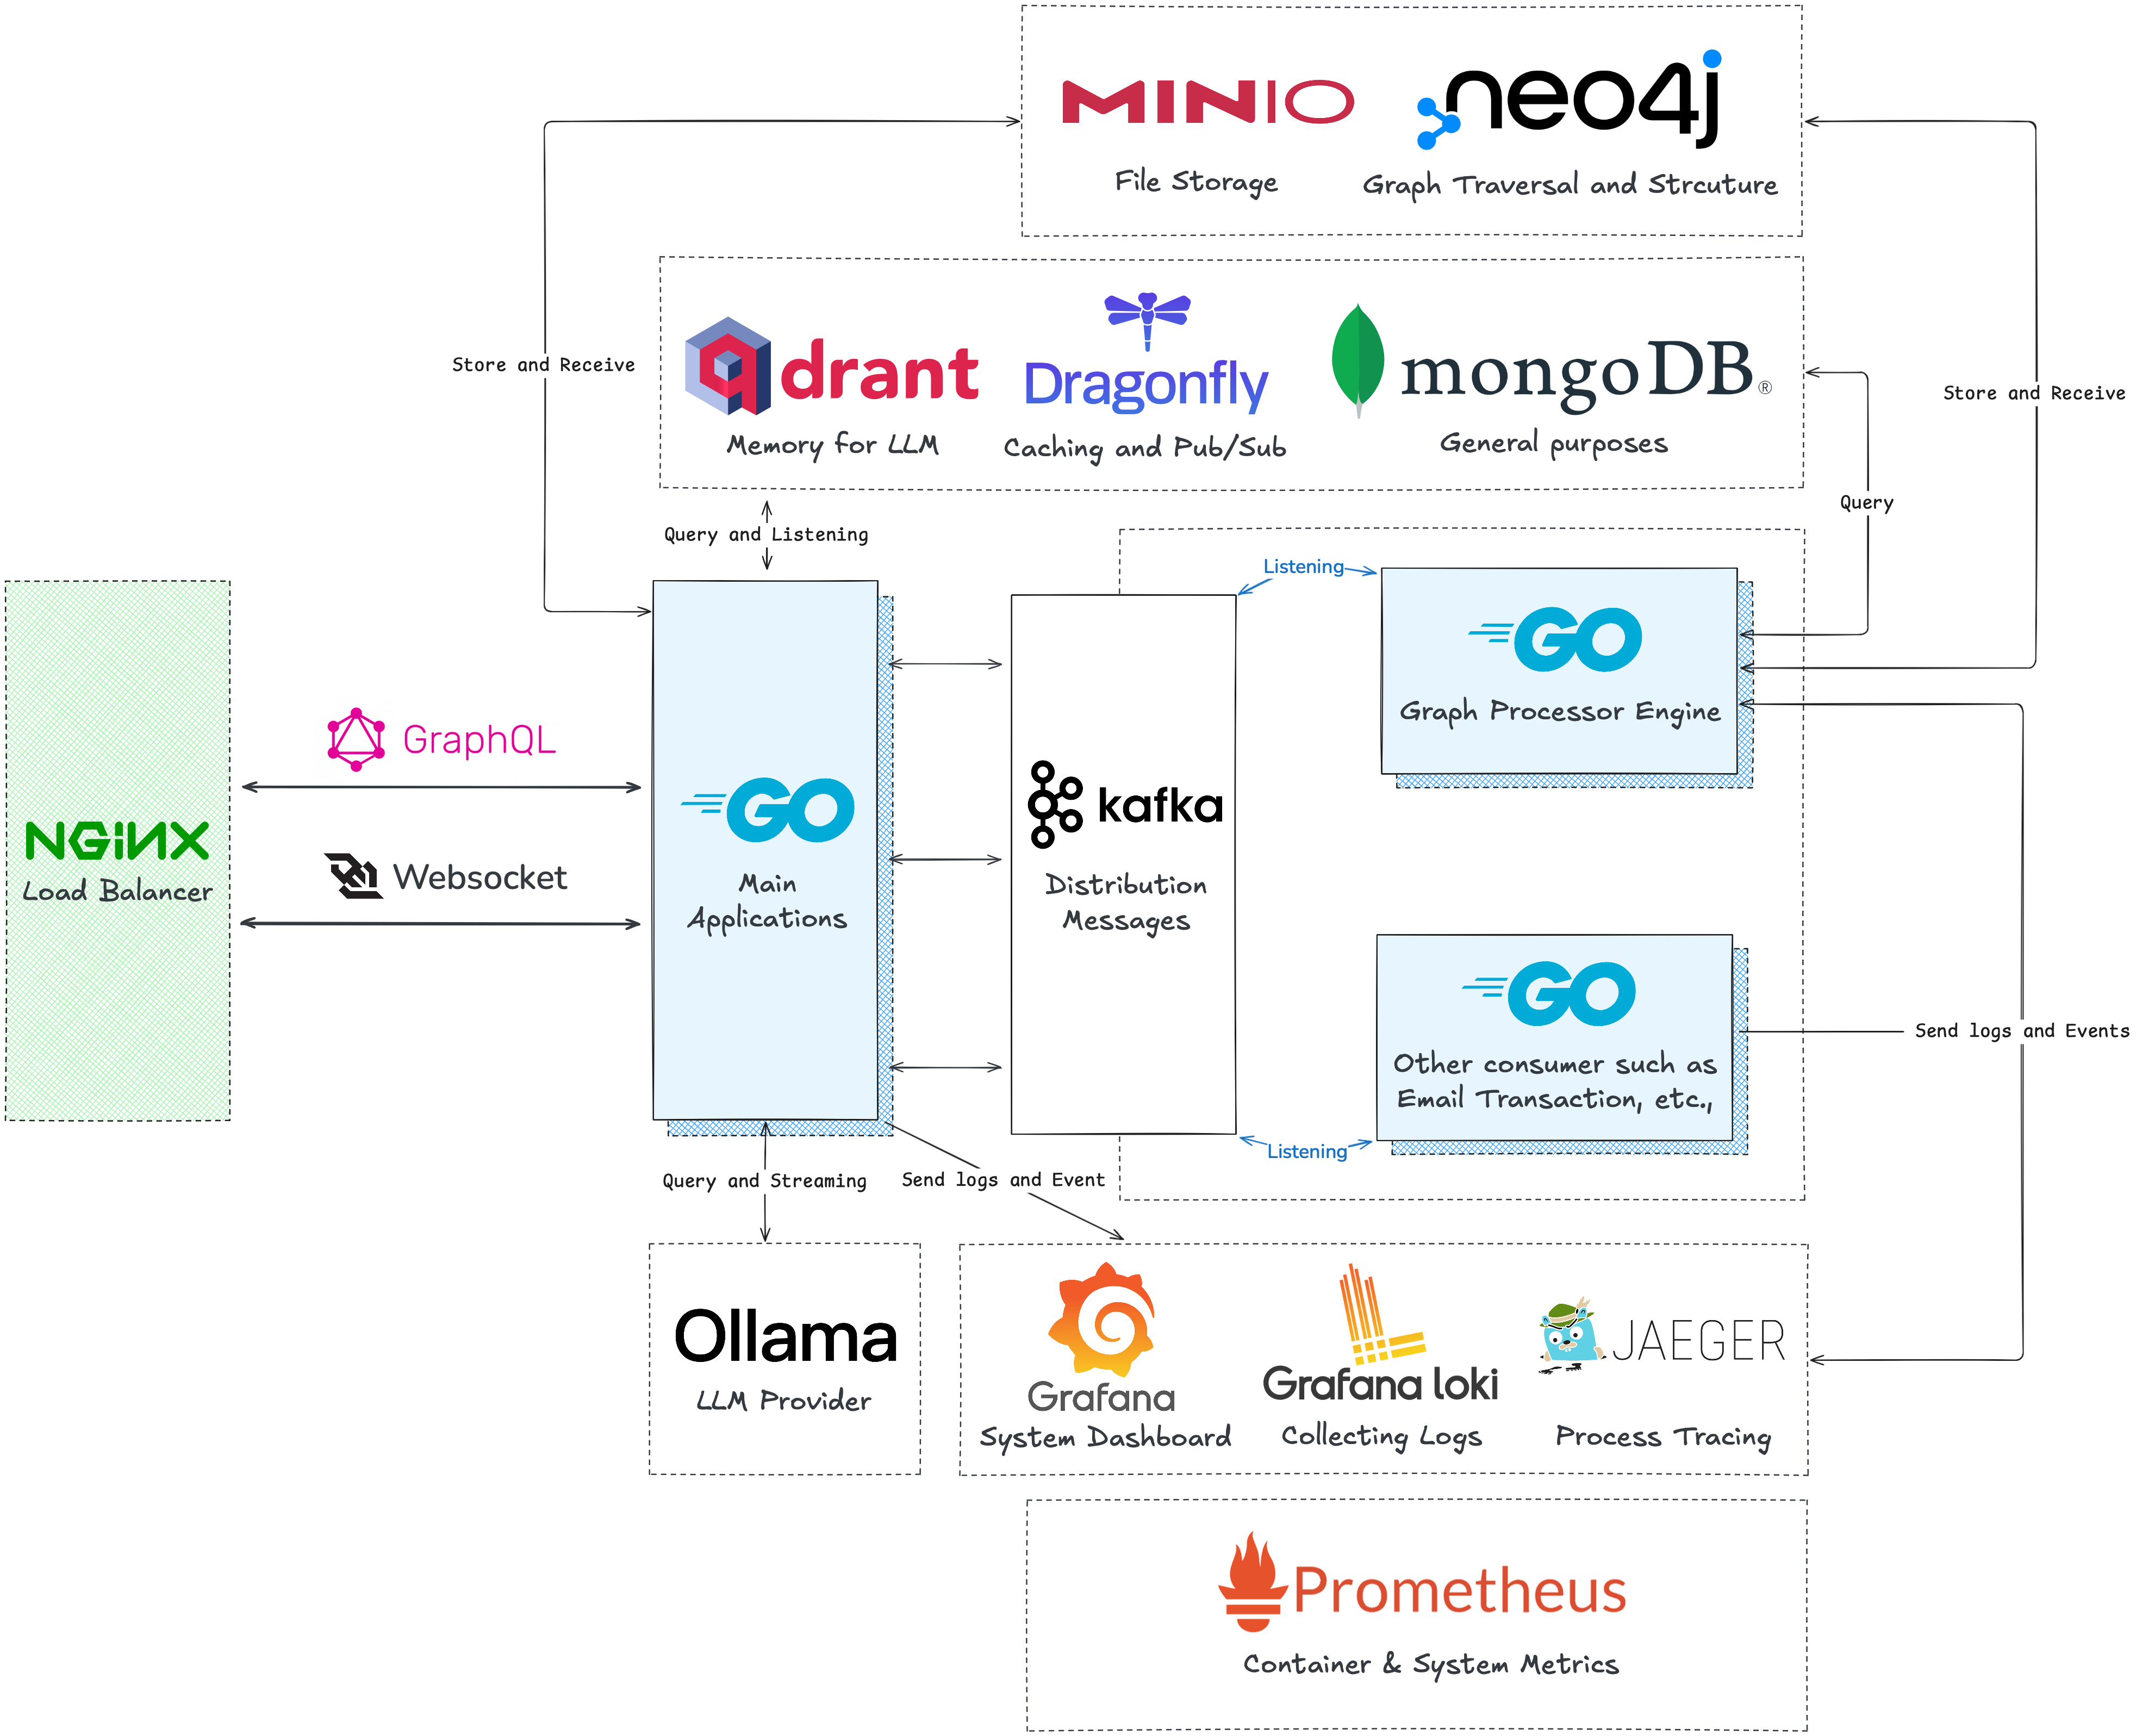
\includegraphics[width=0.8\textwidth]{images/co_occurrence_knowlege_engineering_architecture_diagram.png}
            \caption{สถาปัตยกรรมของแพลตฟอร์มแบบภาพรวม}
            \label{fig:architecture_overview}
        \end{figure}

        \textlight{
            \hspace{1cm}สถาปัตยกรรมของแพลตฟอร์ม Co-Occurrence Knowledge Engineering Platform ได้รับการออกแบบตามหลักการของ Microservices Architecture และ Event-Driven Architecture เพื่อให้สามารถรองรับการประมวลผลข้อมูลขนาดใหญ่และการใช้งานแบบเรียลไทม์ได้อย่างมีประสิทธิภาพ โดยแบ่งองค์ประกอบหลักออกเป็นชั้นต่าง ๆ ดังนี้

            \vspace{0.5cm}

            \textbf{ชั้น Gateway และ Load Balancing}

            \hspace{1cm}\textbf{Nginx (Reverse Proxy \& Load Balancer)} ทำหน้าที่เป็นจุดเข้าถึงหลักของระบบ รับผิดชอบในการกระจายโหลดไปยัง Service ต่าง ๆ และจัดการการเชื่อมต่อจากผู้ใช้งาน โดยรองรับการสื่อสารผ่าน GraphQL API สำหรับการค้นหาและจัดการข้อมูลแบบยืดหยุ่น และ WebSocket สำหรับการสื่อสารแบบเรียลไทม์ เช่น การอัปเดตสถานะการประมวลผลกราฟ การแจ้งเตือน และการซิงโครไนซ์ข้อมูลระหว่างผู้ใช้หลายคน ระบบนี้ยังทำหน้าที่ในการจัดการ SSL/TLS Termination และการรักษาความปลอดภัยในระดับต้น

            \vspace{3.5cm}

            \textbf{ชั้น Application Services}

            \hspace{1cm}\textbf{Main Application (Go)} เป็นแกนหลักของระบบที่เขียนด้วยภาษา Go เพื่อความเร็วและประสิทธิภาพในการประมวลผล รับผิดชอบในการจัดการ Business Logic หลัก เช่น การรับและประมวลผลไฟล์ PDF การวิเคราะห์ Co-occurrence การจัดการผู้ใช้งาน การควบคุมการเข้าถึงข้อมูล และการประสานงานระหว่าง Service ต่าง ๆ ระบบนี้ยังทำหน้าที่ในการส่ง Message ไปยัง Message Queue สำหรับงานที่ต้องการการประมวลผลแบบ Asynchronous

            \hspace{1cm}\textbf{Graph Processor Engine (Go)} เป็น Service พิเศษที่เขียนด้วย Go เพื่อจัดการกับการสร้างและประมวลผลกราฟเครือข่ายขนาดใหญ่ ทำงานแบบ Consumer โดยรับ Message จาก Kafka และประมวลผลการสร้าง Node และ Edge ของกราฟแบบขนานกัน (Parallel Processing) เพื่อให้สามารถจัดการกับข้อมูลขนาดใหญ่ได้อย่างมีประสิทธิภาพ Service นี้มีความสามารถในการ Scale horizontally เมื่อมีปริมาณงานเพิ่มขึ้น

            \hspace{1cm}\textbf{Email Transaction Service (Go)} จัดการกับการส่งอีเมลต่าง ๆ เช่น การยืนยันบัญชีผู้ใช้ การแจ้งเตือนเมื่อการประมวลผลเสร็จสิ้น การส่งรายงานประจำ และการแจ้งเตือนเหตุการณ์สำคัญ โดยทำงานแบบ Asynchronous ผ่าน Message Queue เพื่อไม่ให้กระทบต่อประสิทธิภาพของ Main Application

            \vspace{0.3cm}

            \textbf{ชั้น Message Queue และ Event Streaming}

            \hspace{1cm}\textbf{Apache Kafka} ทำหน้าที่เป็นแกนกลางของ Event-Driven Architecture รับผิดชอบในการรับและกระจาย Message จำนวนมากจาก Main Application ไปยัง Consumer Services ต่าง ๆ โดยเฉพาะงานหนักอย่างการสร้าง Network Graph ขนาดใหญ่ที่จำเป็นต้องแบ่งการประมวลผลออกเป็นหลาย ๆ ส่วน Kafka ช่วยให้ระบบสามารถรองรับ High Throughput และมี Fault Tolerance สูง โดยการจัดเก็บ Message แบบ Persistent และการ Replication ข้ามหลาย Broker

            \vspace{0.3cm}

            \textbf{ชั้นการจัดเก็บข้อมูล (Data Storage Layer)}

            \hspace{1cm}\textbf{Qdrant (Vector Database)} ทำหน้าที่เป็น Memory และ Knowledge Base สำหรับ Large Language Models (LLM) จัดเก็บ Vector Embeddings ของข้อความและแนวคิดต่าง ๆ เพื่อให้ LLM สามารถทำ Semantic Search และ Context-aware Query ได้อย่างมีประสิทธิภาพ ช่วยเพิ่มความแม่นยำในการตอบคำถามและการค้นหาความเชื่อมโยงระหว่างแนวคิด

            \hspace{1cm}\textbf{DragonflyDB (Redis Fork)} เป็นระบบ In-Memory Cache ที่มีประสิทธิภาพสูง ทำหน้าที่ในการ Cache ข้อมูลที่ใช้บ่อย เช่น ผลการค้นหา Session ของผู้ใช้ และข้อมูล Metadata ต่าง ๆ นอกจากนี้ยังทำหน้าที่เป็น Pub/Sub Broker สำหรับการสื่อสารระหว่าง Service แบบเรียลไทม์ และการซิงโครไนซ์ข้อมูลระหว่าง Instance ต่าง ๆ

            \hspace{1cm}\textbf{MongoDB (Document Database)} จัดเก็บข้อมูลทั่วไปของระบบในรูปแบบ Document เช่น ข้อมูลบัญชีผู้ใช้ Metadata ของเอกสาร การตั้งค่าต่าง ๆ ประวัติการใช้งาน และข้อมูล Configuration ต่าง ๆ เหมาะสำหรับข้อมูลที่มีโครงสร้างแบบยืดหยุ่นและต้องการการเข้าถึงที่รวดเร็ว

            \hspace{1cm}\textbf{Neo4j (Graph Database)} เป็นหัวใจสำคัญของระบบที่จัดเก็บ Network Graph ที่เกิดจากการวิเคราะห์ Co-occurrence รวมถึงความสัมพันธ์ระหว่าง Node และ Edge ต่าง ๆ รองรับการ Query แบบ Graph-specific ด้วย Cypher Query Language ทำให้สามารถค้นหารูปแบบความสัมพันธ์ที่ซับซ้อนและการวิเคราะห์ Network Properties ได้อย่างมีประสิทธิภาพ

            \hspace{1cm}\textbf{MinIO (S3-Compatible Object Storage)} จัดเก็บไฟล์ต่าง ๆ ที่ผู้ใช้อัปโหลดเข้าสู่ระบบ เช่น ไฟล์ PDF เอกสารต้นฉบับ รูปภาพที่ส่งออกจากกราฟ และไฟล์ผลลัพธ์ต่าง ๆ รองรับการ Scale แบบ Distributed และมี API ที่เข้ากันได้กับ Amazon S3 ทำให้สามารถ Migrate หรือ Backup ได้ง่าย

            \vspace{0.3cm}

            \textbf{ชั้น AI และ Machine Learning}

            \hspace{1cm}\textbf{Ollama (LLM Service)} ให้บริการ Large Language Models เพื่อการประมวลผลภาษาธรรมชาติ การตีความข้อความ การสร้าง Summary และการตอบคำถามเกี่ยวกับเนื้อหาในกราฟเครือข่าย ทำงานร่วมกับ Qdrant ในการ Retrieve Context ที่เกี่ยวข้องและสร้างคำตอบที่มีความแม่นยำสูง รองรับการ Load Balance และ Scale ตามความต้องการใช้งาน

            \vspace{0.3cm}

            \textbf{ชั้น Observability และ Monitoring}

            \hspace{1cm}\textbf{Grafana Dashboard} เป็นหน้าต่างหลักสำหรับการมองภาพรวมของระบบทั้งหมด แสดงผล Metrics ต่าง ๆ เช่น การใช้งาน CPU, Memory, Network Traffic จำนวนผู้ใช้งาน สถานะของ Service ต่าง ๆ และ Performance Indicators ที่สำคัญ ช่วยให้ผู้ดูแลระบบสามารถติดตามและตัดสินใจได้อย่างรวดเร็ว

            \hspace{1cm}\textbf{Grafana Loki (Log Aggregation)} รวบรวมและจัดการ Log จาก Service ทุกตัวในระบบ ช่วยในการ Debug การวิเคราะห์ปัญหา และการติดตาม Event ต่าง ๆ ที่เกิดขึ้น รองรับการ Query Log แบบ Real-time และการสร้าง Alert เมื่อเกิด Error หรือ Anomaly

            \hspace{1cm}\textbf{Jaeger Tracing} ติดตาม Request Flow ทั้งหมดที่เกิดขึ้นในระบบ แสดง Latency และ Dependencies ระหว่าง Service ต่าง ๆ ช่วยในการ Optimize Performance และการระบุ Bottleneck ในระบบ เป็นเครื่องมือสำคัญสำหรับการ Debug ปัญหาที่เกิดขึ้นใน Microservices Environment

            \hspace{1cm}\textbf{Prometheus (Metrics Collection)} รวบรวมและจัดเก็บ Metrics จาก Service ทุกตัวในระบบ เช่น Response Time, Error Rate, Throughput และ Resource Usage รองรับการสร้าง Alert Rule และการ Integration กับ Grafana สำหรับการแสดงผลแบบ Real-time

            \vspace{0.5cm}

            \textbf{การไหลของข้อมูลและการทำงานของระบบ}

            \hspace{1cm}เมื่อผู้ใช้อัปโหลดเอกสาร PDF ผ่าน Web Interface ข้อมูลจะผ่าน Nginx เข้าสู่ Main Application ซึ่งจะประมวลผลข้อความและส่ง Message ไปยัง Kafka สำหรับการสร้างกราฟ Graph Processor Engine จะรับ Message และสร้าง Node/Edge ใน Neo4j พร้อมทั้งอัปเดต Vector Embeddings ใน Qdrant ผลลัพธ์จะถูก Cache ใน DragonflyDB และผู้ใช้จะได้รับการแจ้งเตือนผ่าน WebSocket เมื่อการประมวลผลเสร็จสิ้น

            \hspace{1cm}ระบบนี้ได้รับการออกแบบให้มีความ Scalable, Fault-tolerant และ Observable ช่วยให้สามารถรองรับการใช้งานระดับ Enterprise และการพัฒนาต่อยอดในอนาคตได้อย่างมีประสิทธิภาพ
        }

        \item[2.10.2] ความสัมพันธ์และแนวคิดข้อมูล (Data Relations and Concepts)
        \\
        \textlight{
            \hspace{1cm}การพัฒนาระบบ Co-Occurrence Knowledge Engineering Platform ต้องอาศัยการทำความเข้าใจเกี่ยวกับโครงสร้างและความสัมพันธ์ของข้อมูลอย่างลึกซึ้ง เนื่องจากระบบนี้มีเป้าหมายในการแปลงข้อความจากเอกสารให้กลายเป็นกราฟเครือข่ายความรู้ที่สามารถแสดงความเชื่อมโยงระหว่างแนวคิดต่าง ๆ ได้อย่างมีความหมาย ดังนั้นจึงจำเป็นต้องมีการออกแบบโครงสร้างข้อมูลและแนวคิดหลักที่รองรับการทำงานของระบบ

            \vspace{0.5cm}

            \textbf{โครงสร้างกราฟเครือข่าย (Network Graph Structure)}

            \hspace{1cm}ในการทำระบบ Knowledge Engineering จำเป็นต้องมี \textbf{Network Graph Structure} เพื่อการค้นหาความเชื่อมโยงระหว่างความรู้อย่างมีประสิทธิภาพ โครงสร้างกราฟเครือข่ายนี้ประกอบด้วยองค์ประกอบหลัก 3 ส่วน ได้แก่

            \begin{enumerate}
                \item[2.10.2.1] \textbf{โหนด (Nodes)} แทนแนวคิด คำศัพท์ หรือเอนทิตีที่สกัดมาจากข้อความ
                \item[2.10.2.2] \textbf{ขอบเชื่อม (Edges)} แทนความสัมพันธ์และความแข็งแกร่งของการเชื่อมโยงระหว่างแนวคิด
                \item[2.10.2.3] \textbf{เซนทรอยด์ (Centroid)} เป็นจุดกึ่งกลางของกราฟทั้งหมด ซึ่งเป็น Concept หลักในการแสดงกราฟทั้งหมด
                
                \vspace{0.3cm}

            \textbf{แนวคิดเซนทรอยด์ (Centroid Concept)}

            \hspace{1cm}\textbf{เซนทรอยด์ (Centroid)} เป็นแนวคิดสำคัญที่ใช้ในการระบุจุดศูนย์กลางหรือแนวคิดหลักของกราฟเครือข่าย โดยเซนทรอยด์จะถูกคำนวณจากความถี่การปรากฏและระดับการเชื่อมโยงของแต่ละโหนดในกราฟ เซนทรอยด์ทำหน้าที่เป็น:

            \begin{enumerate}
                \item[2.10.2.3.1] \textbf{ตัวแทนความหมายหลัก} ของเนื้อหาทั้งหมดในกราฟ
                \item[2.10.2.3.2] \textbf{จุดอ้างอิง} สำหรับการคำนวณความสัมพันธ์กับโหนดอื่น ๆ
                \item[2.10.2.3.3] \textbf{เครื่องมือสรุปเนื้อหา} ที่ช่วยให้เข้าใจแนวคิดหลักได้อย่างรวดเร็ว
                \item[2.10.2.3.4] \textbf{ดัชนีการค้นหา} ที่เพิ่มประสิทธิภาพในการ Query และ Retrieval
            \end{enumerate}

            การคำนวณเซนทรอยด์ใช้อัลกอริทึม Spreading Activation ที่พิจารณาจากค่าน้ำหนักและความเชื่อมโยงของโหนดทั้งหมดในกราฟ

            \vspace{0.3cm}

            \textbf{เงื่อนไขการสร้างกราฟเครือข่าย (Graph Creation Criteria)}

            \hspace{1cm}ในการสร้าง Network Graph สำหรับ Co-occurrence Graph ขึ้นมาได้ จำเป็นต้องมีข้อกำหนดพื้นฐานสำหรับข้อมูลต้นทางและเงื่อนไขทางคณิตศาสตร์ที่ชัดเจน ดังนี้:

            \textbf{เงื่อนไขทางคณิตศาสตร์สำหรับการสร้าง Co-occurrence Graph:}

            \textbf{1. เงื่อนไขความยาวประโยค:}
            
            สำหรับประโยคข้อความ $S$ ที่มีความยาว $n$ คำ จำเป็นต้องมี:
            
            $$n > 0$$
            
            โดยที่ $n$ คือจำนวนคำในประโยคหลังจากการประมวลผล (Tokenization) และการกรอง Stop Words

            \textbf{2. เงื่อนไขการปรากฏร่วม (Co-occurrence Condition):}

            การปรากฏร่วมคือการปรากฏของคำสองคำในประโยคเดียวกัน โดยกำหนดให้:

            สำหรับคำ $w_i$ และ $w_j$ ใน corpus $C$ ที่มีการปรากฏร่วมกันด้วยความถี่ $f(w_i, w_j)$

            $$f(w_i, w_j) \geq \sigma$$

            โดยที่:
            
            $f(w_i, w_j)$ = ความถี่การปรากฏร่วมของคำ $w_i$ และ $w_j$ ในประโยคเดียวกัน
            
            $\sigma$ = ค่าเกณฑ์ขั้นต่ำ (threshold) สำหรับการปรากฏร่วมที่มีนัยสำคัญ
            
            กำหนดให้ $\sigma = 2$ สำหรับระบบนี้

            \vspace{6cm}

            \textbf{3. เงื่อนไขการสร้างขอบเชื่อม (Edge Creation Condition):}

            ขอบเชื่อม $e_{ij}$ ระหว่างโหนด $w_i$ และ $w_j$ จะถูกสร้างขึ้นก็ต่อเมื่อ:

            $$e_{ij} = \begin{cases} 
            1, & \text{ถ้า } f(w_i, w_j) \geq \sigma \\
            0, & \text{ถ้า } f(w_i, w_j) < \sigma 
            \end{cases}$$

            \textbf{4. น้ำหนักของขอบเชื่อม (Edge Weight):}

            น้ำหนักของขอบเชื่อม $w_{ij}$ คำนวณจาก:

            $$w_{ij} = \frac{f(w_i, w_j)}{\max_{k,l \in V} f(w_k, w_l)}$$

            โดยที่ $V$ คือเซตของโหนดทั้งหมดในกราฟ

            \textbf{5. เงื่อนไขการกรองข้อมูล (Data Filtering Condition):}

            เมื่อกำหนด $\sigma = 2$ แล้ว ข้อความใดที่มีความถี่การปรากฏร่วมต่ำกว่าค่านี้จะไม่ถูกนำมาสร้างกราฟ กล่าวคือ:

            $$\forall (w_i, w_j) : f(w_i, w_j) < 2 \Rightarrow (w_i, w_j) \notin E$$

            โดยที่ $E$ คือเซตของขอบเชื่อมทั้งหมดในกราฟ

            \textbf{6. เงื่อนไขการคำนวณ Centroid:}

            สำหรับการคำนวณ Centroid ของกราฟ ใช้สูตร:

            $$C = \sum_{w_j \in V} w_{ij} \cdot d_{ij}^{-1}$$

            โดยที่:
            \begin{itemize}
                \item $C$ = Centroid ของกราฟ
                \item $d_{ij}$ = ระยะทางสั้นที่สุดระหว่างโหนด $w_i$ และ $w_j$
                \item $V$ = เซตของโหนดทั้งหมดที่ผ่านเงื่อนไขความถี่
            \end{itemize}

            \textbf{7. เงื่อนไขความหนาแน่นของกราฟ (Graph Density Condition):}

            ความหนาแน่นของกราฟ $D$ คำนวณจาก:

            $$D = \frac{2|E|}{|V|(|V|-1)}$$

            โดยที่:
            \begin{itemize}
                \item $|E|$ = จำนวนขอบเชื่อมที่มีความถี่ $\geq \sigma$
                \item $|V|$ = จำนวนโหนดทั้งหมดในกราฟ
            \end{itemize}

            \vspace{5cm}

            \textbf{8. ตัวอย่างการประยุกต์ใช้:}

            ให้ประโยค: "ระบบวิศวกรรมความรู้ช่วยในการวิเคราะห์ข้อมูล"

            หลังจาก Tokenization และ Stop Words Removal: ["ระบบ", "วิศวกรรม", "ความรู้", "วิเคราะห์", "ข้อมูล"]

            Co-occurrence pairs ที่เป็นไปได้:
            \begin{itemize}
                \item (ระบบ, วิศวกรรม), (ระบบ, ความรู้), (ระบบ, วิเคราะห์), (ระบบ, ข้อมูล)
                \item (วิศวกรรม, ความรู้), (วิศวกรรม, วิเคราะห์), (วิศวกรรม, ข้อมูล)
                \item (ความรู้, วิเคราะห์), (ความรู้, ข้อมูล)
                \item (วิเคราะห์, ข้อมูล)
            \end{itemize}

            เฉพาะ pairs ที่มี $f(w_i, w_j) \geq 2$ เท่านั้นที่จะถูกนำมาสร้างเป็นขอบเชื่อมในกราฟ

            \textbf{กระบวนการสร้างกราฟ:}

            \begin{enumerate}
                \item[2.10.2.4.1] \textbf{การแบ่งคำ (Tokenization)} แยกประโยคออกเป็นคำแต่ละคำ
                \item[2.10.2.4.2] \textbf{การกรองคำ (Filtering)} กำจัด Stop Words และคำที่ไม่มีความหมาย
                \item[2.10.2.4.3] \textbf{การสร้างโหนด (Node Creation)} แปลงคำที่เหลือเป็นโหนดในกราฟ
                \item[2.10.2.4.4] \textbf{การคำนวณ Co-occurrence} วิเคราะห์การปรากฏร่วมของคำ
                \item[2.10.2.4.5] \textbf{การสร้างขอบเชื่อม (Edge Creation)} เชื่อมโยงโหนดตามค่า Co-occurrence
            \end{enumerate}

            \vspace{0.3cm}

            \textbf{การจัดเก็บ Metadata และ Context}

            \hspace{1cm}สำหรับทุกคำที่ถูกแปลงเป็นโหนดในกราฟ ระบบจะสร้างและจัดเก็บ \textbf{Metadata} ที่สำคัญดังนี้:

            \begin{enumerate}
                \item[2.10.2.5.1] \textbf{ข้อความประโยคต้นฉบับ (Original Sentences)} เก็บประโยคเดิมที่คำนั้น ๆ เคยปรากฏอยู่
                \item[2.10.2.5.2] \textbf{ตำแหน่งในเอกสาร (Document Position)} บันทึกหน้า บรรทัด และตำแหน่งของคำ
                \item[2.10.2.5.3] \textbf{ความถี่การปรากฏ (Frequency)} นับจำนวนครั้งที่คำปรากฏในเอกสาร
                \item[2.10.2.5.4] \textbf{บริบทโดยรอบ (Surrounding Context)} เก็บคำ ๆ ข้างเคียงเพื่อสร้าง Context Window
                \item[2.10.2.5.5] \textbf{ข้อมูลการประมวลผล (Processing Metadata)} เก็บข้อมูลเกี่ยวกับวิธีการประมวลผลและ Algorithm ที่ใช้
            \end{enumerate}

            Metadata เหล่านี้จะถูกนำไปใช้เป็น \textbf{Context} ให้กับ Large Language Models (LLM) เพื่อการ:

            \begin{enumerate}
                \item[2.10.2.5.6] \textbf{Context-Aware Question Answering} ตอบคำถามโดยอิงจากบริบทที่ถูกต้อง
                \item[2.10.2.5.7] \textbf{Semantic Understanding} เข้าใจความหมายของคำในบริบทต่าง ๆ
                \item[2.10.2.5.8] \textbf{Knowledge Discovery} ค้นพบความรู้ใหม่จากการเชื่อมโยงบริบท
                \item[2.10.2.5.9] \textbf{Content Summarization} สร้างสรุปเนื้อหาที่มีความหมาย
            \end{enumerate}

            \vspace{0.3cm}

            \textbf{ความสัมพันธ์ระหว่างข้อมูล (Data Relationships)}

            \hspace{1cm}ระบบใช้หลายรูปแบบความสัมพันธ์เพื่อแสดงการเชื่อมโยงระหว่างข้อมูล:

            \begin{enumerate}
                \item[2.10.2.6.1] \textbf{Co-occurrence Relationship} ความสัมพันธ์จากการปรากฏร่วมในข้อความ
                \item[2.10.2.6.2] \textbf{Semantic Relationship} ความสัมพันธ์เชิงความหมาย โดยใช้ Vector Embeddings
                \item[2.10.2.6.3] \textbf{Hierarchical Relationship} ความสัมพันธ์แบบลำดับชั้น จากการจัดหมวดหมู่
                \item[2.10.2.6.4] \textbf{Temporal Relationship} ความสัมพันธ์เชิงเวลา จากลำดับการปรากฏ
                \item[2.10.2.6.5] \textbf{Contextual Relationship} ความสัมพันธ์จากบริบทที่ใช้งาน
            \end{enumerate}

            \vspace{0.3cm}

            \textbf{โมเดลข้อมูลสำหรับระบบ (Data Model)}

            \hspace{1cm}ระบบใช้โมเดลข้อมูลแบบ Hybrid ที่ผสมผสานหลายแนวทาง:

            \textbf{Graph Data Model:}
            \begin{itemize}
                \item Nodes: แทนแนวคิดและเอนทิตี
                \item Edges: แทนความสัมพันธ์และน้ำหนัก
                \item Properties: แทน Metadata และ Attributes
            \end{itemize}

            \textbf{Vector Data Model:}
            \begin{itemize}
                \item Embeddings: แทนความหมายเชิงลึกของข้อความ
                \item Similarity Scores: แทนความคล้ายคลึงทางความหมาย
                \item Clustering Information: แทนการจัดกลุ่มตามความหมาย
            \end{itemize}

            \textbf{Document Data Model:}
            \begin{itemize}
                \item Original Text: เก็บข้อความต้นฉบับ
                \item Processed Text: เก็บข้อความหลังประมวลผล
                \item Metadata: เก็บข้อมูลเสริมและการประมวลผล
            \end{itemize}

            \vspace{0.5cm}

            \textbf{การประยุกต์ใช้แนวคิดในระบบ}

            \hspace{1cm}แนวคิดเหล่านี้ถูกนำไปประยุกต์ใช้ในระบบเพื่อสร้างประสบการณ์การใช้งานที่มีประสิทธิภาพ ได้แก่:

            \begin{enumerate}
                \item[2.10.2.7.1] \textbf{Intelligent Search} การค้นหาที่เข้าใจบริบทและความหมาย
                \item[2.10.2.7.2] \textbf{Dynamic Visualization} การแสดงผลกราฟที่ปรับตัวตามข้อมูล
                \item[2.10.2.7.3] \textbf{Pattern Discovery} การค้นพบรูปแบบและแนวโน้มใหม่
                \item[2.10.2.7.4] \textbf{Knowledge Fusion} การผสมผสานความรู้จากหลายแหล่ง
                \item[2.10.2.7.5] \textbf{Automated Insights} การสร้าง Insights อัตโนมัติจากข้อมูล
            \end{enumerate}

            \hspace{1cm}ความสำคัญของการออกแบบโครงสร้างข้อมูลและแนวคิดเหล่านี้คือ ช่วยให้ระบบสามารถจัดการกับความซับซ้อนของความรู้และสร้างความเข้าใจที่ลึกซึ้งจากข้อมูลที่มีอยู่ ทำให้ผู้ใช้งานสามารถค้นพบความเชื่อมโยงและสร้างความรู้ใหม่ได้อย่างมีประสิทธิภาพ

            \end{enumerate}
        }

        \vspace{10cm}

        \item[2.10.3] เส้นทางข้อมูลการสร้างกราฟ (Graph Creation Data Flow)

        \begin{figure}[H]
            \centering
            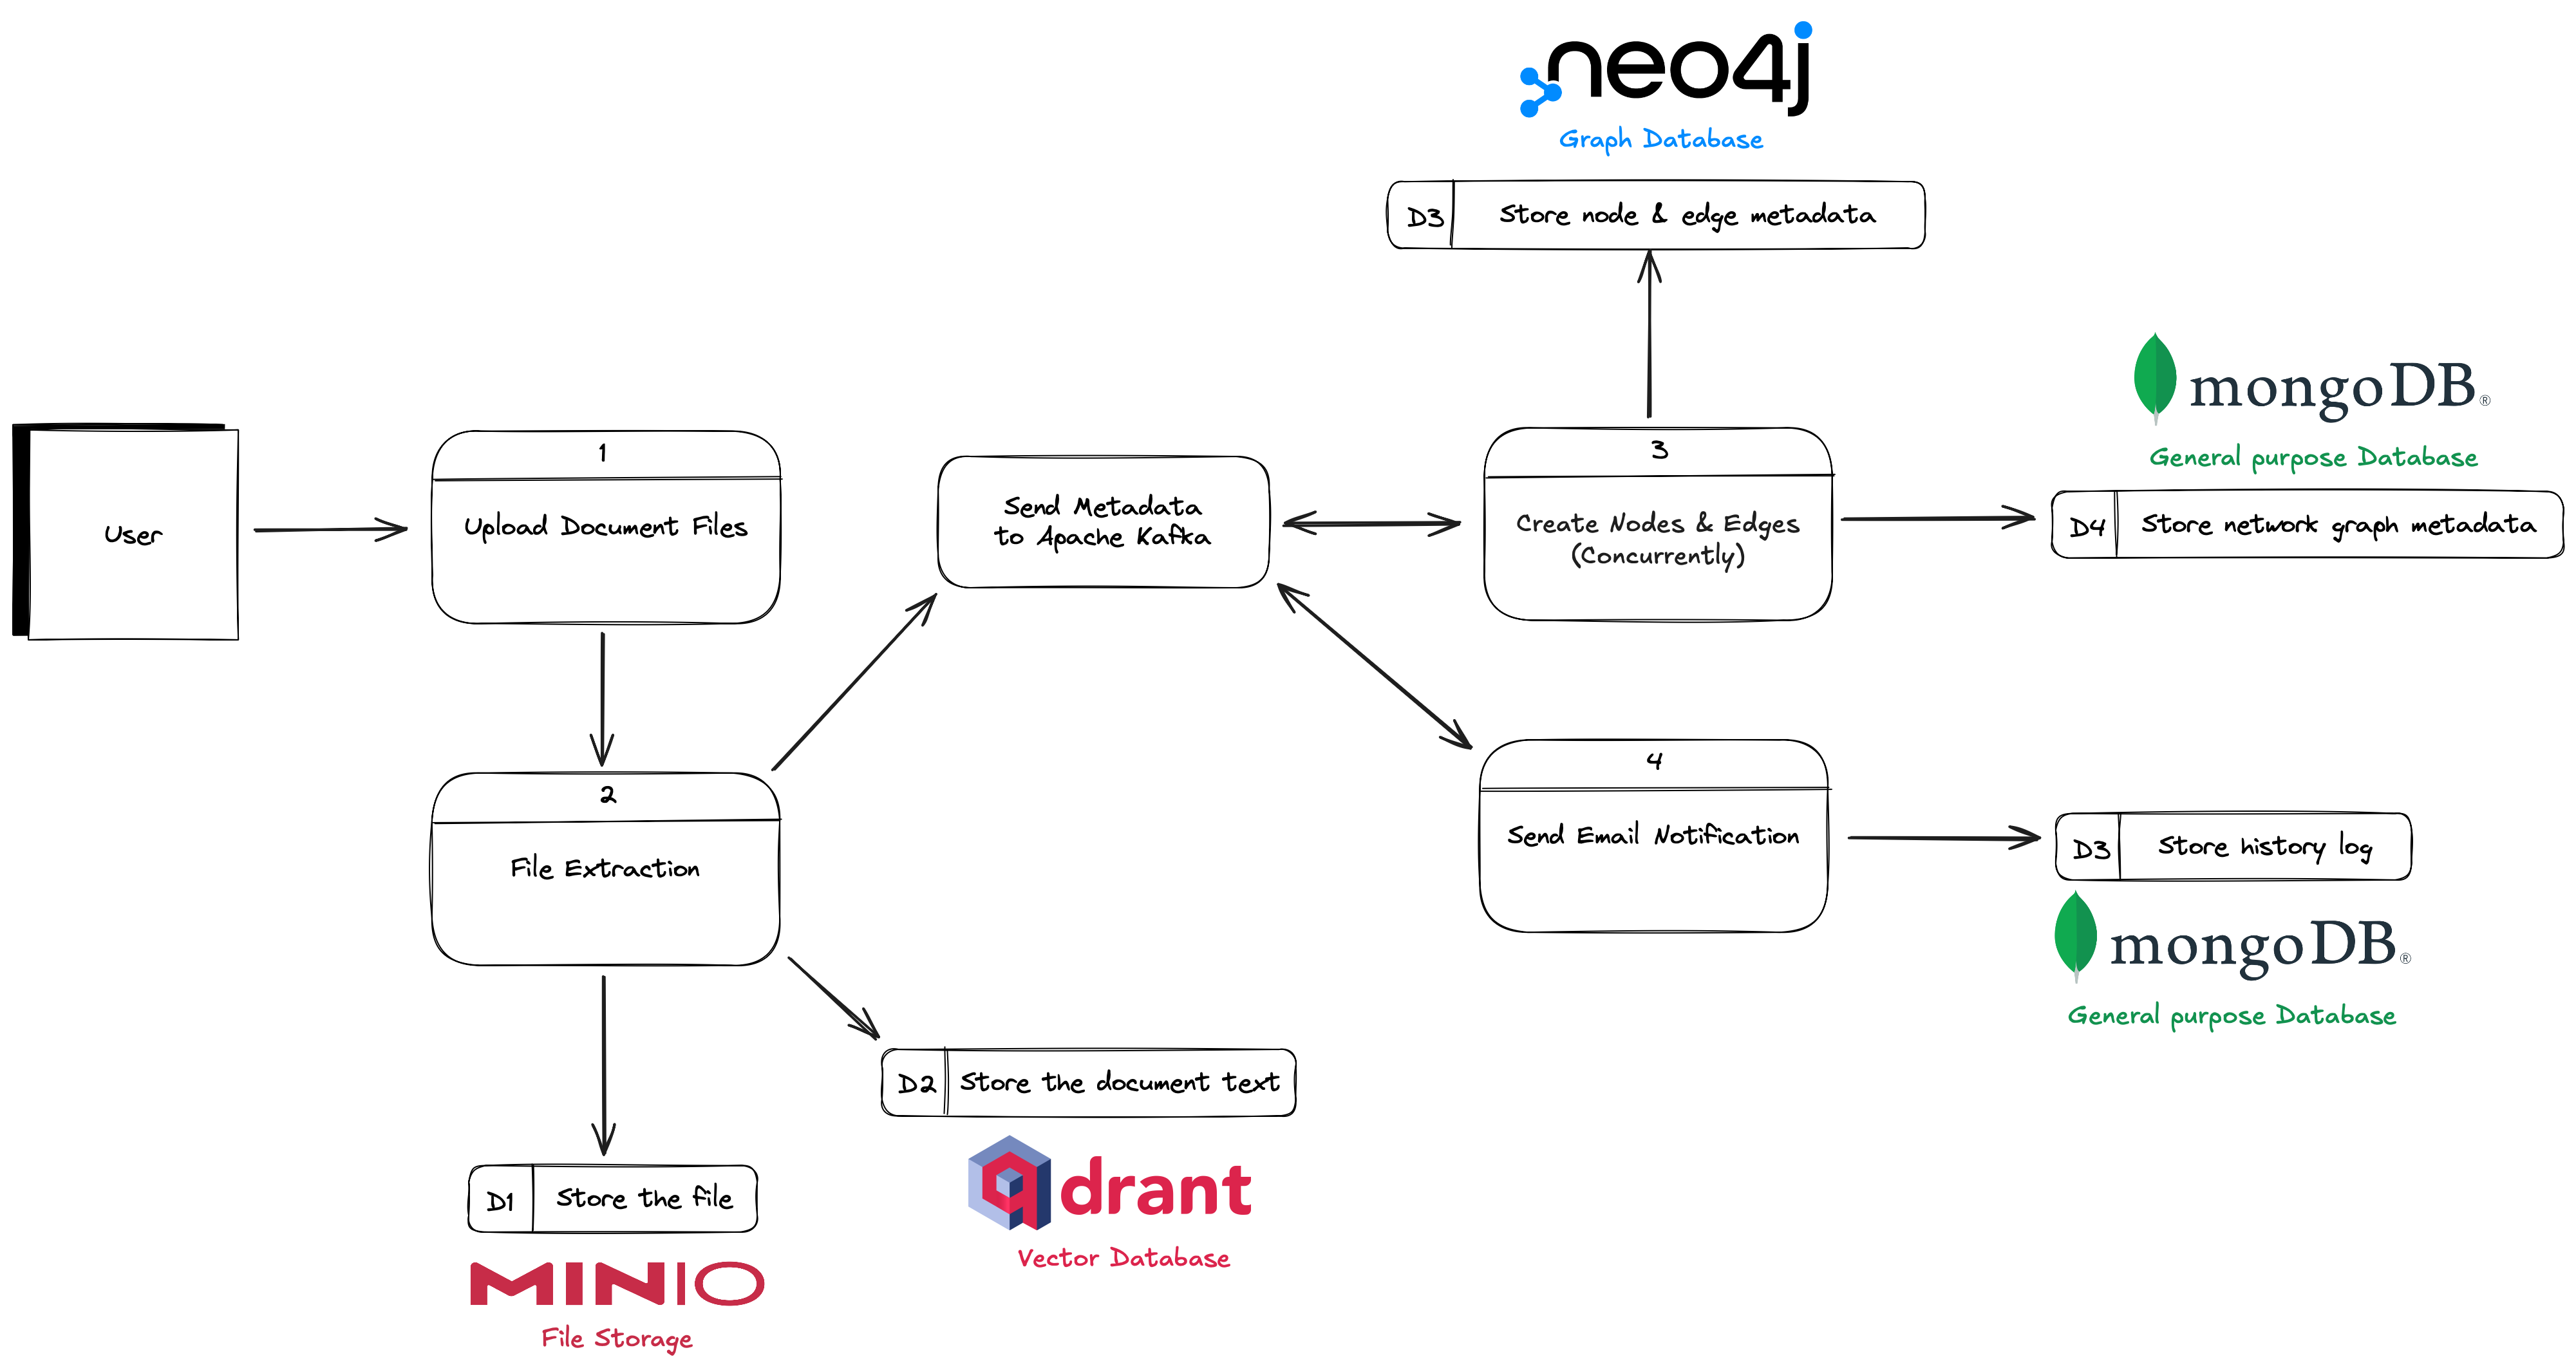
\includegraphics[width=0.8\textwidth]{images/co-p-data_flow_concept.png}
            \caption{เส้นทางข้อมูลการสร้างกราฟของแพลตฟอร์ม}
            \label{fig:data_flow_concept}
        \end{figure}

        \textlight{
            \hspace{1cm}เส้นทางข้อมูลการสร้างกราฟของแพลตฟอร์ม Co-Occurrence Knowledge Engineering Platform ได้รับการออกแบบให้มีความสะดวก เป็นระบบ และมีประสิทธิภาพในการจัดการข้อมูลจำนวนมาก โดยใช้หลักการของ \textbf{Event-Driven Architecture} และ \textbf{Microservices} เพื่อให้สามารถประมวลผลข้อมูลแบบ Asynchronous และ Scale ได้ตามปริมาณงาน ขั้นตอนการทำงานของระบบมีดังนี้:

            \vspace{0.5cm}

            \textbf{ขั้นตอนที่ 1: การอัปโหลดเอกสารจากผู้ใช้ (Document Upload)}

            \hspace{1cm}ผู้ใช้งานเริ่มต้นกระบวนการโดยการอัปโหลดไฟล์เอกสาร โดยเฉพาะไฟล์ PDF ผ่านทาง Web Interface ของแพลตฟอร์ม ระบบจะทำการตรวจสอบความถูกต้องของไฟล์ เช่น ขนาดไฟล์ รูปแบบไฟล์ และความสมบูรณ์ของข้อมุล หลังจากการตรวจสอบเสร็จสิ้น ไฟล์จะถูกส่งผ่าน \textbf{Nginx Load Balancer} เข้าสู่ระบบ Backend เพื่อเริ่มขั้นตอนการประมวลผล การออกแบบนี้ช่วยให้ระบบสามารถรองรับการอัปโหลดไฟล์หลายไฟล์พร้อมกันได้อย่างมีประสิทธิภาพ

            \vspace{0.3cm}

            \textbf{ขั้นตอนที่ 2: การสกัดข้อความจากเอกสาร (Text Extraction)}

            \hspace{1cm}เมื่อไฟล์เอกสารเข้าสู่ระบบ Backend แล้ว \textbf{Main Application} จะทำการสกัดข้อความ (Text Extraction) จากไฟล์ PDF โดยใช้ \textbf{PDF Text Parsing} สำหรับเอกสารที่มีข้อความดิจิทัล ระบบจะทำการจัดการกับเลย์เอาต์ที่ซับซ้อน การแยกส่วนหัวข้อ เนื้อหา และส่วนอ้างอิง รวมถึงการจัดการกับภาษาไทยที่มีลักษณะการเว้นวรรคและการตัดคำที่แตกต่างจากภาษาอังกฤษ ผลลัพธ์ที่ได้จะเป็นข้อความที่สะอาดและพร้อมสำหรับการวิเคราะห์ขั้นต่อไป

            \vspace{0.3cm}

            \textbf{ขั้นตอนที่ 3: การจัดเก็บข้อมูลในระบบหลายชั้น (Multi-tier Data Storage)}

            \hspace{1cm}ข้อมูลที่ผ่านการประมวลผลแล้วจะถูกจัดเก็บในระบบที่มีหลายชั้น ได้แก่ \textbf{MinIO Object Storage} สำหรับเก็บไฟล์ต้นฉบับและไฟล์ที่เกี่ยวข้อง เช่น รูปภาพที่สกัดจากเอกสาร Metadata ต่าง ๆ และ \textbf{Qdrant Vector Database} สำหรับจัดเก็บ \textbf{Vector Embeddings} ของข้อความ ซึ่งจะใช้ในการทำ \textbf{Semantic Search} และการให้บริการ \textbf{Large Language Models (LLM)} ในขั้นตอนต่อไป การแยกการจัดเก็บข้อมูลแบบนี้ช่วยให้ระบบสามารถเข้าถึงข้อมูลได้รวดเร็วและมีประสิทธิภาพตามการใช้งานที่แตกต่างกัน

            \vspace{0.3cm}

            \textbf{ขั้นตอนที่ 4: การส่งข้อมูลผ่าน Message Queue (Batch Processing via Kafka)}

            \hspace{1cm}เพื่อให้ระบบสามารถจัดการกับข้อมูลจำนวนมากได้อย่างมีประสิทธิภาพ ระบบจะส่งข้อมูลไปยัง \textbf{Apache Kafka Message Queue} แบบทีละ Batch ซึ่งช่วยในการจัดการกับข้อมูลที่มีปริมาณมากโดยไม่ทำให้ระบบล่มหรือตอบสนองช้า Kafka ทำหน้าที่เป็น \textbf{Event Streaming Platform} ที่รองรับการประมวลผลแบบ \textbf{Asynchronous} และมี \textbf{Fault Tolerance} สูง โดยสามารถกู้คืนข้อมูลได้ในกรณีที่เกิดปัญหา การออกแบบนี้ช่วยให้ระบบสามารถรองรับการใช้งานจำนวนมากพร้อมกันได้โดยไม่ส่งผลกระทบต่อประสิทธิภาพ

            \vspace{0.3cm}

            \textbf{ขั้นตอนที่ 5: การสร้าง Node และ Edge Metadata พร้อมการแจ้งเตือน (Graph Construction \& Notification)}

            \hspace{1cm}\textbf{Graph Processor Engine} ที่เขียนด้วยภาษา Go จะทำหน้าที่เป็น \textbf{Consumer} รับข้อมูลจาก Kafka แล้วประมวลผลการสร้าง \textbf{Node และ Edge} ของกราฟเครือข่าย โดยใช้อัลกอริทึม \textbf{Co-occurrence Analysis} ในการคำนวณความสัมพันธ์ระหว่างคำและแนวคิดต่าง ๆ ข้อมูล Metadata ที่สร้างขึ้นจะถูกจัดเก็บใน \textbf{Neo4j Graph Database} เพื่อการค้นหาและวิเคราะห์ความสัมพันธ์แบบกราฟ ในขณะเดียวกัน ระบบจะส่ง \textbf{Email Notification} ผ่าน \textbf{Email Transaction Service} เพื่อแจ้งให้ผู้ใช้ทราบเมื่อการประมวลผลเสร็จสิ้น และจัดเก็บ \textbf{History Log} ลงใน \textbf{MongoDB} เพื่อการติดตามและการตรวจสอบประวัติการทำงานของระบบ

            \vspace{0.3cm}

            \textbf{ขั้นตอนที่ 6: การจัดเก็บ Network Graph และการเตรียมพร้อมใช้งาน (Graph Storage \& Optimization)}

            \hspace{1cm}หลังจากการสร้างกราฟเครือข่ายเสร็จสิ้น ข้อมูล \textbf{Network Graph} ทั้งหมดจะถูกจัดเก็บใน \textbf{MongoDB} ในรูปแบบที่เหมาะสำหรับการเรียกใช้งานในครั้งถัดไป โดยการจัดเก็บจะรวมถึง \textbf{Graph Metadata, Node Properties, Edge Weights, และ Visualization Settings} ต่าง ๆ ระบบจะทำการ \textbf{Indexing} และ \textbf{Optimization} เพื่อให้การเข้าถึงข้อมูลมีความรวดเร็ว นอกจากนี้ ข้อมูลที่ใช้บ่อยจะถูก Cache ลงใน \textbf{DragonflyDB (Redis Fork)} เพื่อเพิ่มประสิทธิภาพในการตอบสนอง และระบบจะส่งสัญญาณผ่าน \textbf{WebSocket} เพื่อแจ้งให้ผู้ใช้ทราบว่าข้อมูลพร้อมใช้งานแล้ว

            \vspace{0.5cm}

            \textbf{ข้อดีของการออกแบบเส้นทางข้อมูลแบบนี้}

            \begin{enumerate}
                \item[1.] \textbf{ประสิทธิภาพสูง (High Performance):} การใช้ Event-Driven Architecture ช่วยให้ระบบสามารถประมวลผลข้อมูลแบบขนานกันได้ ลดเวลาในการรอ
                \item[2.] \textbf{ความทนทานต่อข้อผิดพลาด (Fault Tolerance):} Kafka และ Message Queue ช่วยให้ระบบสามารถกู้คืนได้เมื่อเกิดปัญหา
                \item[3.] \textbf{ความสามารถในการขยายตัว (Scalability):} สามารถเพิ่ม Consumer และ Worker ได้ตามปริมาณงานที่เพิ่มขึ้น
                \item[4.] \textbf{การแยกความรับผิดชอบ (Separation of Concerns):} แต่ละ Service มีหน้าที่เฉพาะ ทำให้ง่ายต่อการพัฒนาและบำรุงรักษา
                \item[5.] \textbf{การติดตามและควบคุม (Monitoring \& Observability):} ระบบมี Logging, Metrics และ Tracing ครบถ้วนผ่าน Grafana, Loki, Jaeger และ Prometheus
            \end{enumerate}

            \vspace{0.7cm}

            \textbf{การประยุกต์ใช้กับ Large Language Models (LLM)}

            \hspace{1cm}ข้อมูลที่จัดเก็บใน Vector Database (Qdrant) และ Graph Database (Neo4j) จะถูกนำไปใช้กับ \textbf{Ollama LLM Service} เพื่อการทำ \textbf{Retrieval-Augmented Generation (RAG)} ทำให้ LLM สามารถตอบคำถามและให้ข้อมูลที่แม่นยำขึ้นโดยอิงจากบริบทจากกราฟเครือข่ายที่สร้างขึ้น การรวมกันนี้ช่วยให้ผู้ใช้งานสามารถค้นหาความรู้และทำความเข้าใจความเชื่อมโยงระหว่างแนวคิดต่าง ๆ ได้อย่างลึกซึ้งและมีประสิทธิภาพ
        }
    \end{enumerate}

    \vspace{1cm}

    \textlight{
        ภาพตัวอย่างของแพลตฟอร์ม Co-Occurrence Knowledge Engineering Platform ที่แสดงให้เห็นถึงการทำงานและความสามารถของระบบ โดยจะแบ่งออกเป็น 2 ภาพหลัก ได้แก่ กราฟขนาดใหญ่ที่แสดงความสัมพันธ์ระหว่างเอกสารและกราฟขนาดเล็กที่แสดงความสัมพันธ์ระหว่างแนวคิดต่าง ๆ ในเอกสาร
    }

    \begin{figure}[H]
        \centering
        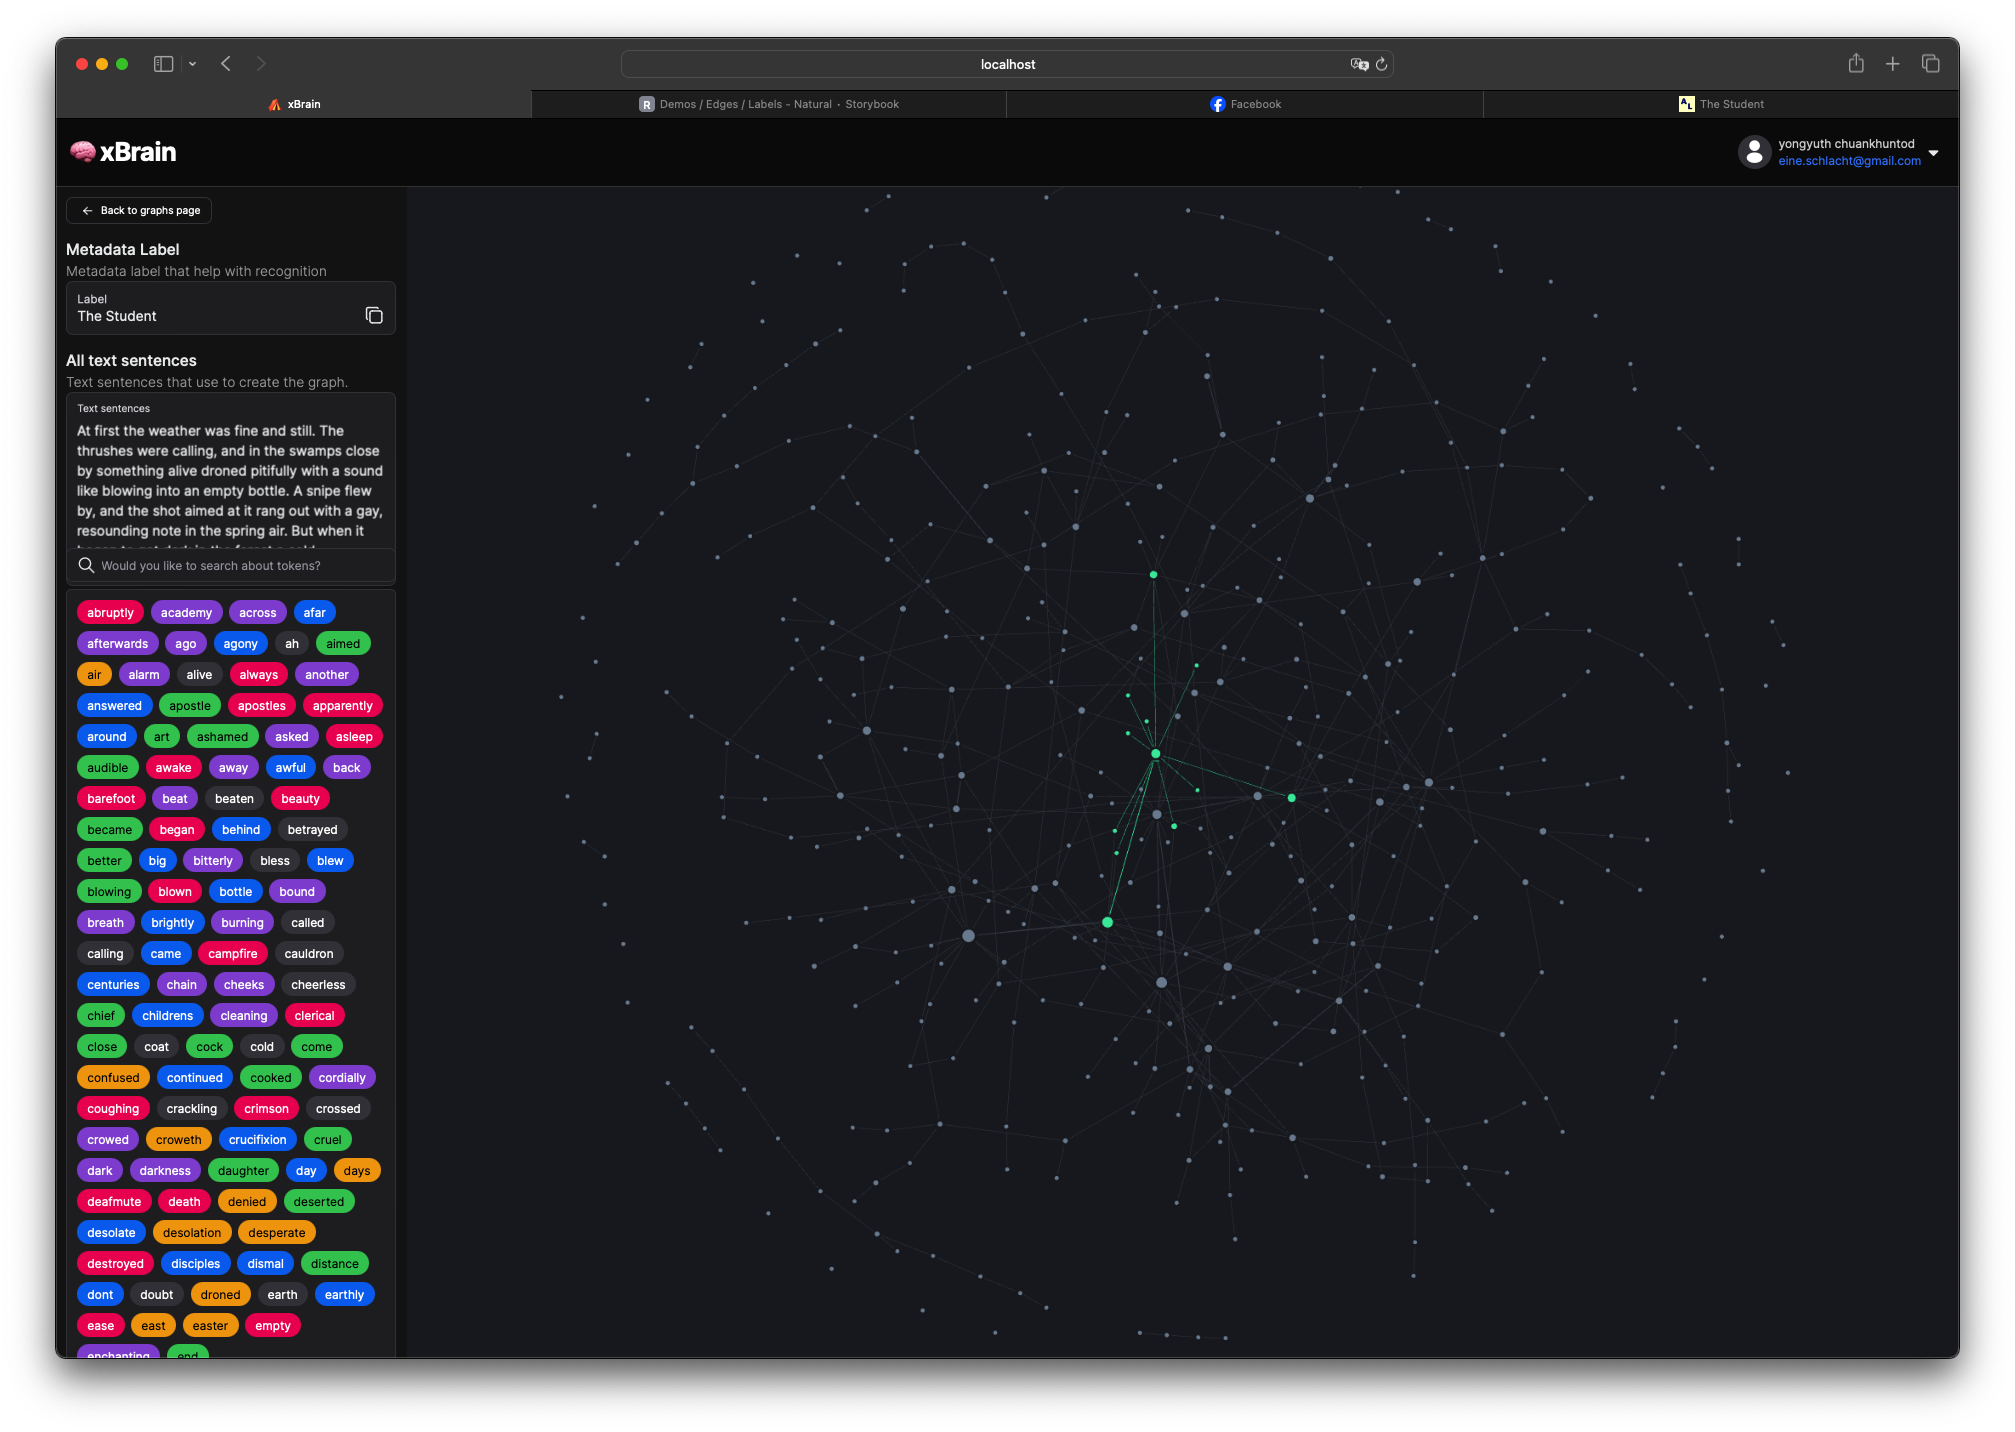
\includegraphics[width=0.8\textwidth]{images/platform_1.png}
        \caption{กราฟขนาดใหญ่ที่แสดงความสัมพันธ์}
        \label{fig:platform_1}
    \end{figure}

\end{enumerate}

\vspace{5cm}

\hfill\begin{minipage}{10cm}
    \vspace{0.5cm}
    \begin{center}
        \textlight{ลงชื่อ \dotrule{150pt} ผู้เสนอโครงการ}\\[0.2cm]
        \textlight{(\dotrule{180pt})}\\[0.4cm]
        \textlight{วันที่ \dotrule{50pt}/\dotrule{50pt}/\dotrule{50pt}}
    \end{center}
    \vspace{0.5cm}
\end{minipage}         

\vspace{0.5cm}

\textlight{ความเห็นอาจารย์ที่ปรึกษา}
\dotrule{378pt}

\dotrule{500pt}

\dotrule{500pt}

\vspace{0.5cm}

\hfill\begin{minipage}{10cm}
    \vspace{0.5cm}
    \begin{center}
        \textlight{ลงชื่อ \dotrule{150pt} อาจารย์ที่ปรึกษา}\\[0.2cm]
        \textlight{(\dotrule{180pt})}\\[0.4cm]
        \textlight{วันที่ \dotrule{50pt}/\dotrule{50pt}/\dotrule{50pt}}
    \end{center}
    \vspace{0.5cm}
\end{minipage}                          

\vspace{13cm}

\textlight{สาขาวิชา / ภาควิชาที่ได้รับแบบเสนอโครงงานวันนี้ \dotrule{260pt}}

\textlight{ผลการพิจารณา}
\dotrule{422pt}

\dotrule{500pt}

\dotrule{500pt}

\vspace{2cm}

\hfill\begin{minipage}{8cm}
    \vspace{0.5cm}
    \begin{center}
        \textlight{ลงชื่อ \dotrule{150pt} ประธาน}\\[0.2cm]
        \textlight{(\dotrule{180pt})}\\[0.4cm]
        \textlight{วันที่ \dotrule{50pt}/\dotrule{50pt}/\dotrule{50pt}}
    \end{center}
    \vspace{0.5cm}
\end{minipage}  

\hfill\begin{minipage}{8cm}
    \vspace{0.5cm}
    \begin{center}
        \textlight{ลงชื่อ \dotrule{150pt} กรรมการ}\\[0.2cm]
        \textlight{(\dotrule{180pt})}\\[0.4cm]
        \textlight{วันที่ \dotrule{50pt}/\dotrule{50pt}/\dotrule{50pt}}
    \end{center}
    \vspace{0.5cm}
\end{minipage}

\hfill\begin{minipage}{8cm}
    \vspace{0.5cm}
    \begin{center}
        \textlight{ลงชื่อ \dotrule{150pt} กรรมการ}\\[0.2cm]
        \textlight{(\dotrule{180pt})}\\[0.4cm]
        \textlight{วันที่ \dotrule{50pt}/\dotrule{50pt}/\dotrule{50pt}}
    \end{center}
    \vspace{0.5cm}
\end{minipage}

\hfill\begin{minipage}{8cm}
    \vspace{0.5cm}
    \begin{center}
        \textlight{ลงชื่อ \dotrule{150pt} กรรมการ}\\[0.2cm]
        \textlight{(\dotrule{180pt})}\\[0.4cm]
        \textlight{วันที่ \dotrule{50pt}/\dotrule{50pt}/\dotrule{50pt}}
    \end{center}
    \vspace{0.5cm}
\end{minipage}

\end{document}
